\subsection{局部凸空间上的 Mackey 拓扑与弱化拓扑}

设 E 为局部凸空间，\(E'\) 为其对偶。我们将 E 与 \(E'\) 置于对偶，所借助的典范双线性型为 \((x, x') \mapsto \langle x, x' \rangle\)，它定义在 \(E \times E'\) 上。这一对偶在 \(E'\) 中是分离的。我们将考虑 E 上与 E 和 \(E'\) 之间的对偶相容的三种拓扑：

\begin{enumerate}
\def\labelenumi{\alph{enumi})}
\item
  E 上原先给定的拓扑，当可能产生混淆时，我们称其为初始拓扑；
\item
  拓扑 \(\sigma(\mathrm{E},\mathrm{E}^{\prime})\)，称为 \(\mathrm{E}\) 上的弱化拓扑；
\item
  拓扑 \(\tau(\mathrm{E},\mathrm{E}')\)，称为 E 上的 Mackey 拓扑。
\end{enumerate}

初始拓扑比弱化拓扑细，而比 Mackey 拓扑粗；此外，这三种拓扑可以互不相同（IV，第 49 页，习题 8）。

由 IV 第 1 页的命题 1，这三种拓扑具有相同的闭凸集、相同的桶、相同的有界集以及相同的适配有界结构。特别地：

命题 2. --- 设 E 为局部凸空间，A 为 E 的一个凸子集（例如 E 的一个向量子空间）。A 对于 E 的初始拓扑的闭包与对于 E 的弱化拓扑的闭包相同。

注. --- 1) E 中元素的一族 \((x_{i})_{i\in\mathbf{I}}\) 对于初始拓扑是完全的（相应地，拓扑无关的），当且仅当它对于弱化拓扑也是如此；这由命题 2 得出。因此我们可以应用 II 第 43 页的判别法。

\begin{enumerate}
\def\labelenumi{\arabic{enumi})}
\setcounter{enumi}{1}
\tightlist
\item
  设 \(\mathcal{T}_1\) 与 \(\mathcal{T}_2\) 是 E 上的两个局部凸拓扑，与 E 和 E' 之间的对偶相容，且 \(\mathcal{T}_1\) 比 \(\mathcal{T}_2\) 细。则 0 的每个对于 \(\mathcal{T}_1\) 的邻域，只要它是凸的且对于 \(\mathcal{T}_1\) 闭，就对于 \(\mathcal{T}_2\) 闭（依据 IV 第 1 页的命题 1）。因此（GT, II, § 3, 第 3 目，推论）E 中每个对于 \(\mathcal{T}_2\) 完备的子集对于 \(\mathcal{T}_1\) 也完备。
\end{enumerate}

特别地，E 中每个对于弱化拓扑完备的子集对于初始拓扑完备，而 E 中每个对于初始拓扑完备的子集对于 Mackey 拓扑也完备。若 E 对于弱化拓扑拟完备，则它对于每个与 E 和 E' 之间的对偶相容的拓扑都如此。若它对于初始拓扑拟完备，则它对于 Mackey 拓扑也如此。

\begin{enumerate}
\def\labelenumi{\arabic{enumi})}
\setcounter{enumi}{2}
\tightlist
\item
  假定 E 是 Hausdorff 的（对初始拓扑而言）。设 A 是 E 的一个子集，它对于 \(\sigma(\mathrm{E}, \mathrm{E}')\) 闭且有界，从而对于每个与 E 和 \(E'\) 之间的对偶相容的拓扑也如此。由于 A 对于 \(\sigma(\mathrm{E}, \mathrm{E}')\) 预紧（III，第 3 页，注 5），假定 A 对于 \(\sigma(\mathrm{E}, \mathrm{E}')\) 紧等价于 A 对于 \(\sigma(\mathrm{E}, \mathrm{E}')\) 完备。
\end{enumerate}

因此，根据注 2，我们看出：

命题 3. --- 假定 E 是 Hausdorff 的，E' 是它的对偶。E 中每个对于初始拓扑预紧且对于 \(\sigma(E, E')\) 紧的子集，对于初始拓扑是紧的。

\begin{enumerate}
\def\labelenumi{\arabic{enumi})}
\setcounter{enumi}{3}
\tightlist
\item
  拓扑 \(\beta(\mathrm{E},\mathrm{E}')\)（IV，第 4 页，定义 3）比 Mackey 拓扑细。若 \(\beta(\mathrm{E},\mathrm{E}')\) 不同于 \(\tau(\mathrm{E},\mathrm{E}')\)，则它与 E 和 E' 之间的对偶不相容。E 是桶型空间当且仅当初始拓扑等于 \(\beta(\mathrm{E},\mathrm{E}')\)（III，第 24 页）。
\end{enumerate}

命题 4. --- 设 E 为局部凸空间。在下列每种情形中，E 上的 Mackey 拓扑都与初始拓扑相同：

\begin{enumerate}
\def\labelenumi{\alph{enumi})}
\item
  E 是桶型空间；
\item
  E 是有界型空间；
\item
  E 是可度量化的。
\end{enumerate}

我们首先注意到，E 上的 Mackey 拓扑与初始拓扑相同，当且仅当 \(E'\) 的每个对于 \(\sigma(E', E)\) 紧的凸子集都是等度连续的。当 E 是桶型空间时情形当然如此（III，第 24 页，推论）。

设 E 是有界型空间；令 V 是 E 中对于拓扑 \(\tau(E, E')\) 的一个凸均衡零邻域。令 B 是 E 的一个对于初始拓扑有界的子集。由于 B 对于 Mackey 拓扑有界，V 吸收 B；又由于 E 是有界型空间，V 是对于初始拓扑的零邻域。

在情形 c)，空间 E 是有界型的（III，第 12 页，命题 2）。

\subsection{连续线性映射的转置}

在本节中，\(E_{1}\) 与 \(E_{2}\) 表示两个局部凸空间，其对偶分别为 \(E_{1}^{\prime}\) 与 \(E_{2}^{\prime}\)。

设 \(u\) 是从 \(\mathrm{E}_1\) 到 \(\mathrm{E}_2\) 中的线性映射。为使 \(u\) 在 \(\mathrm{E}_1\) 与 \(\mathrm{E}_2\) 赋予弱化拓扑后连续，必要且充分的是：\(f \circ u\) 属于 \(\mathrm{E}_1'\)（对每个 \(f \in \mathrm{E}_2'\)）；若 \(u\) 连续，则此条件成立。于是，线性映射 \(f \mapsto f \circ u\)（它把 \(\mathrm{E}_2'\) 映到 \(\mathrm{E}_1'\) 中）称为 \(u\) 的转置，记作 \(^t u\)。

命题 5. --- 设 u 是从 \(E_{1}\) 到 \(E_{2}\) 中的连续线性映射。

\begin{enumerate}
\def\labelenumi{(\roman{enumi})}
\item
  若 \(E_{1}\) 与 \(E_{2}\) 是 Hausdorff 的，则 u 为单射当且仅当 \(^{t}u\) 的像在 \(E_{1}^{\prime}\) 中对于弱拓扑 \(\sigma(\mathrm{E}_{1}^{\prime},\mathrm{E}_{1})\) 稠密。
\item
  为使 \({}^{t}u\) 单射，必要且充分的是 \(u\) 的像在 \(\mathbf{E}_2\) 中稠密。
\end{enumerate}

\(E_{2}\) 的向量子空间对于初始拓扑稠密，当且仅当它对于弱化拓扑稠密（IV，第 4 页，命题 2）。于是命题 5 由 II 第 47 页的推论 2 得出。

命题 6. --- 设 u 是从 \(E_{1}\) 到 \(E_{2}\) 中的线性映射，且它对于弱化拓扑连续。对 i = 1, 2，设 \(S_{i}\) 是 \(E_{i}\) 的有界子集的一个族。为使 \(^{t}u\) 是从 \((\mathrm{E}_{2}^{\prime})_{\mathfrak{S}_{2}}\) 到 \((\mathrm{E}_{1}^{\prime})_{\mathfrak{S}_{1}}\) 中的连续映射，必要且充分的是：对每个集 \(A \in S_{1}\)，存在集 \(A_{1}, \ldots, A_{n}\)（均属于 \(S_{2}\)）以及一个实数 \(\lambda > 0\)，使得 \(\lambda.u(\mathbf{A})\) 包含在 \(A_{1} \cup \ldots \cup A_{n}\) 的闭均衡凸包中。

这是 III 第 15 页命题 2 的直接推论。

推论. --- 设 u 是从 \(E_{1}\) 到 \(E_{2}\) 中的连续线性映射。则 \({}^t u\) 在对偶空间 \(E_{i}'\) 赋以下列拓扑时连续：

\begin{enumerate}
\def\labelenumi{\alph{enumi})}
\item
  弱拓扑 \(\sigma (\mathrm{E}_i^{\prime},\mathrm{E}_i)\)
\item
  强拓扑 \(\beta (\mathrm{E}_i^{\prime},\mathrm{E}_i)\)
\item
  Mackey 拓扑 \(\tau (\mathrm{E}_i^{\prime},\mathrm{E}_i)\)
\item
  预紧收敛拓扑。
\end{enumerate}

此外，若 \(E_{2}\) 是 Hausdorff 的，则 \(^{t}u\) 在对偶空间 \(E_{i}^{\prime}\) 赋以下列拓扑时连续：

\begin{enumerate}
\def\labelenumi{\alph{enumi})}
\setcounter{enumi}{4}
\tightlist
\item
  紧收敛拓扑（相应地，紧凸收敛拓扑）。
\end{enumerate}

唯一需要证明的是情形 \(c\)），即 \(\mathrm{E}_1\) 与 \(\mathrm{E}_2\) 的拓扑未必为 Hausdorff 的情况。此时，对每个线性型 \(f \in \mathrm{E}'_1{}^*\)，\(f \circ {}^t u\) 是 \(\mathrm{E}_2'\) 上的线性型；于是存在线性映射 \(v: \mathrm{E}'_1{}^* \to \mathrm{E}'_2{}^*\)，它对于拓扑 \(\sigma(\mathrm{E}'_1{}^*, \mathrm{E}'_1)\) 与 \(\sigma(\mathrm{E}'_2{}^*, \mathrm{E}'_2)\) 连续，且满足 \(d_{\mathrm{B}_2} \circ u = v \circ d_{\mathrm{B}_1}\)，其中 \(d_{\mathrm{B}_i}\) 是从 \(\mathrm{E}_i\) 到 \(\mathrm{E}'_i{}^* (i = 1, 2)\) 中的典范映射。因此，若 A 是 \(\mathrm{E}_1\) 的子集，且 \(d_{\mathrm{B}_1}(\mathrm{A})\) 对于 \(\sigma(\mathrm{E}'_1{}^*, \mathrm{E}'_1)\) 是凸、均衡且紧的，则 \(d_{\mathrm{B}_2}(u(\mathrm{A})) = v(d_{\mathrm{B}_1}(\mathrm{A}))\) 对于 \(\sigma(\mathrm{E}'_2{}^*, \mathrm{E}'_2)\) 是凸、均衡且紧的，因为拓扑 \(\sigma(\mathrm{E}'_1{}^*, \mathrm{E}'_1)\) 与 \(\sigma(\mathrm{E}'_2{}^*, \mathrm{E}'_2)\) 都是 Hausdorff 的。

命题 7. --- 设 \(u: \mathrm{E}_1 \to \mathrm{E}_2\) 是线性映射。我们假定 \(u\) 对于 \(\mathrm{E}_1\) 与 \(\mathrm{E}_2\) 的弱化拓扑连续。

\begin{enumerate}
\def\labelenumi{(\roman{enumi})}
\item
  映射 \(u\) 在 \(\mathrm{E}_1\) 与 \(\mathrm{E}_2\) 赋予各自的 Mackey 拓扑时是连续的。
\item
  若 \(\mathbf{E}_1\) 是有界型的或桶型的，则 \(u\) 对于 \(\mathbf{E}_1\) 与 \(\mathbf{E}_2\) 的初始拓扑连续。
\item
  为使 \(u\) 对于 \(\mathbf{E}_1\) 与 \(\mathbf{E}_2\) 的初始拓扑连续，必要且充分的是：在 \(^t u\) 之下，\(\mathbf{E}_2'\) 的每个等度连续子集的像在 \(\mathbf{E}_1'\) 中等度连续。
\end{enumerate}

该假设蕴含 \({}^t u\) 对于弱拓扑 \(\sigma(\mathrm{E}_2', \mathrm{E}_2)\) 与 \(\sigma(\mathrm{E}_1', \mathrm{E}_1)\) 连续（II，第 46 页，推论），因此 \({}^t u\) 将对于 \(\sigma(\mathrm{E}_2', \mathrm{E}_2)\) 凸、均衡且紧的子集映为对于 \(\sigma(\mathrm{E}_1', \mathrm{E}_1)\) 凸、均衡且紧的集，这是因为拓扑 \(\sigma(\mathrm{E}_2', \mathrm{E}_2)\) 与 \(\sigma(\mathrm{E}_1', \mathrm{E}_1)\) 都是 Hausdorff 的。于是，断言 (i) 由 GT，X，§ 1，第 4 目，命题 3，b) 得出。断言 (ii) 是 (i) 的推论：因为若 \(\mathrm{E}_1\) 是有界型的或桶型的，则其初始拓扑就是 Mackey 拓扑，而 \(\mathrm{E}_2\) 的 Mackey 拓扑比 \(\mathrm{E}_2\) 的初始拓扑细。最后，\(\mathrm{E}_i\) 的初始拓扑是在 \(\mathrm{E}_i'\) 的等度连续子集上一致收敛的拓扑（III，第 19 页，命题 7 的推论 1）。这就证明了 (iii)。

推论. --- 设 \(E_{1}\) 是赋范空间。设 u 是从 \(E_{1}\) 到 \(E_{2}\) 中的线性映射。下列性质等价：

\begin{enumerate}
\def\labelenumi{\alph{enumi})}
\item
  \(u\) 连续；
\item
  \(u\) 对于弱化拓扑连续；
\item
  \(\mathrm{E}_1\) 中单位球在 \(u\) 下的像在 \(\mathrm{E}_2\) 中有界；
\item
  对每个点列 \((x_{n})\)（由 \(\mathbf{E}_1\) 中对于初始拓扑趋于 0 的点构成），序列 \((u(x_{n}))\) 对于 \(\mathbf{E}_2\) 的弱化拓扑有界。
\end{enumerate}

由于 \(E_{1}\) 是有界型的，a) 与 b) 的等价性由命题 7 得出；a) 与 c) 的等价性是显然的。a) 与 d) 的等价性由 IV 第 1 页的命题 1 以及 III 第 11 页的命题 1 得出。

命题 8. --- (i) 设 E 是赋范空间，其对偶为 E'。对每个 \(x \in E\)，我们有

\[
\| x \| = \sup _ {x ^ {\prime} \in \mathrm{E} ^ {\prime}, \| x ^ {\prime} \| \leqslant 1} | \langle x, x ^ {\prime} \rangle |.\tag{3}
\]

\begin{enumerate}
\def\labelenumi{(\roman{enumi})}
\setcounter{enumi}{1}
\tightlist
\item
  设 \(\mathbf{E}_1\) 与 \(\mathbf{E}_2\) 是两个赋范空间，\(u\) 是从 \(\mathbf{E}_1\) 到 \(\mathbf{E}_2\) 中的连续线性映射。我们有
\end{enumerate}

\[
\left\| ^ {t} u \right\| = \left\| u \right\|.\tag{4}
\]

设 \(x \in E\)。对每个 \(x' \in E'\)（满足 \(\| x' \| \leqslant 1\)），我们有

\[
\left| \langle x, x ^ {\prime} \rangle \right| \leqslant \| x \| \| x ^ {\prime} \| \leqslant \| x \|.
\]

由 Hahn-Banach 定理（II，第 23 页，推论 2），存在元素 \(x'\)（属于 \(E'\)），使得 \(\| x' \| \leqslant 1\) 且 \(\langle x, x' \rangle = \| x \|\)。这就证明了 (i)。

现在证明 (ii)。由公式 (3) 以及转置的定义，我们有

\[
\begin{array}{l} \| ^ {t} u \| = \sup _ {\| y ^ {\prime} \| \leqslant 1} \left\| ^ {t} u (y ^ {\prime}) \right\| = \sup _ {\| y ^ {\prime} \| \leqslant 1, \| x \| \leqslant 1} \left| \langle x, ^ {t} u (y ^ {\prime}) \rangle \right| \\ = \sup _ {\| x \| \leqslant 1, \| y ^ {\prime} \| \leqslant 1} \left| \langle u (x), y ^ {\prime} \rangle \right| = \sup _ {\| x \| \leqslant 1} \left\| u (x) \right\| = \| u \|. \end{array}
\]

注. --- 1) 公式 (3) 是 (4) 的特殊情形，对应于从 K 到 E 中的线性映射 \(\lambda \mapsto \lambda x\)。

\begin{enumerate}
\def\labelenumi{\arabic{enumi})}
\setcounter{enumi}{1}
\tightlist
\item
  令 \(\mathrm{B}(x, y') = \langle u(x), y' \rangle = \langle x, {}^t u(y') \rangle\)（其中 \(x \in \mathrm{E}_1\)，\(y' \in \mathrm{E}_2'\)）。上述证明表明 \(\mathbf{B}\) 是 \(\mathrm{E}_1 \times \mathrm{E}_2'\) 上的连续双线性型，其范数（GT，X，§ 3，第 2 目）等于 \(\| u \|\)。
\end{enumerate}

推论. --- 设 E 是满足第一可数公理的赋范空间。存在 \(E' - \{0\}\) 的可数子集 D，使得我们有

\[
\| x \| = \sup _ {\xi \in \mathbf {D}} | \langle x, \xi \rangle | / \| \xi \|\tag{5}
\]

对所有 \(x \in E\) 成立。

设 \(B'\) 是对偶 \(E'\)（即 \(E\) 的对偶）的单位球，并对其赋予弱拓扑 \(\sigma(E', E)\)。则 \(B'\) 是紧度量空间（III，第 19 页，推论 2）；因此存在可数稠密子集 \(D'\)（在 \(B'\) 中）。令 \(D = D' \cap (E' - \{0\})\)。设 \(x \in E\)；映射 \(x' \mapsto \langle x, x' \rangle\)（它把 \(B'\) 映到 \(K\) 中）连续，因此

\[
\sup _ {x ^ {\prime} \in \mathbf {B} ^ {\prime}} | \langle x, x ^ {\prime} \rangle | = \sup _ {\xi \in \mathbf {D} ^ {\prime}} | \langle x, \xi \rangle | \leqslant \sup _ {\xi \in \mathbf {D}} | \langle x, \xi \rangle | / \| \xi \| \leqslant \| x \|.
\]

于是公式 (5) 由 (3) 得出。

\subsection{商空间与子空间的对偶}

在本节中，E 表示一个局部凸空间，M 表示 E 的一个向量子空间，而 \(M^{\circ}\) 表示 M 在 E 的对偶 \(E'\) 中的正交集。设 p 是从 E 到 E/M 上的典范映射；则 \(^{t}p\) 是单射的，其像为 \(M^{\circ}\)，从而定义一个向量空间同构（非拓扑的）

\[
\pi : (\mathrm{E} / \mathbf {M}) ^ {\prime} \rightarrow \mathbf {M} ^ {\circ}.
\]

类似地，设 i 是从 M 到 E 中的典范单射。则 \({}^{t}i\) 是满射的（II，第 24 页，命题 2）；其核等于 \(M^{\circ}\)，于是我们得到一个向量空间同构（非拓扑的）

\[
\iota : \mathrm{E} ^ {\prime} / \mathrm{M} ^ {\circ} \rightarrow \mathrm{M} ^ {\prime}.
\]

命题 9. --- (i) 为使 (E/M)' 的子集 A 等度连续，必要且充分的是 \(\pi(A)\) 是 \(E'\) 的等度连续子集。

\begin{enumerate}
\def\labelenumi{(\roman{enumi})}
\setcounter{enumi}{1}
\item
  设 \(\mathfrak{S}\) 是 E 的有界子集组成的一个集，\(\mathfrak{S}_1\) 是诸子集 \(\mathrm{A} \in \mathfrak{S}\) 在 E/M 中的像组成的集。则 \(\pi\) 是从 \((\mathrm{E} / \mathrm{M})_{\mathfrak{S}_1}'\) 到 \(\mathbf{M}^\circ\) 上的一个同构，其中 \(\mathbf{M}^\circ\) 赋予由 \(\mathrm{E}_{\mathfrak{S}}'\) 的拓扑诱导的拓扑。
\item
  设 E 是赋范空间，则 \(\pi\) 是从赋范空间 (E/M)' 到 E' 的赋范子空间 M° 上的一个等距。
\end{enumerate}

设 A 是 \((\mathrm{E}/\mathrm{M})'\) 的子集，\(\mathbf{B} = {}^{t}p(\mathbf{A}) \subset \mathbf{E}'\)。令

\[
q (\xi) = \sup _ {\xi^ {\prime} \in \mathbf {A}} | \langle \xi , \xi^ {\prime} \rangle |
\]

对所有 \(\xi \in \mathrm{E} / \mathbf{M}\) 成立。为使 A 等度连续，必要且充分的是：映射 \(q\)（从 \(\mathrm{E} / \mathbf{M}\) 到 \(\overline{\mathbf{R}}_+\) 中）是连续半范数。这蕴含 \(q \circ p\) 是 \(\mathrm{E}\) 上的连续半范数（II，第 27 页，命题 5，(ii)）。由于我们有

\[
(q \circ p) (x) = \sup _ {x ^ {\prime} \in \mathbf {B}} | \langle x, x ^ {\prime} \rangle |
\]

对所有 \(x \in E\) 成立，而这又蕴含 B 在 \(E'\) 中等度连续，于是 (i) 得证。设 \(A \in S\)，f 是 E/M 上的连续线性型。对每个 \(\lambda \in R_{+}\)，\(|f| \leqslant \lambda\) 在 \(p(A)\) 上成立当且仅当 \(|^{t}p(f)| \leqslant \lambda\) 在 A 上成立；由此得 (ii)。

最后证明 (iii)。设 \(y'\) 属于 \((\mathrm{E} / \mathbf{M})'\)。\(\mathrm{E} / \mathbf{M}\) 中一个元素的范数 \(< 1\)，当且仅当它是 \(p\) 下某个元素的像，该元素具有范数 \(< 1\) 且位于 \(\mathbf{E}\) 中。于是

\[
\begin{array}{l} \| y ^ {\prime} \| = \sup _ {y \in \mathrm{E} / \mathbf {M}, \| y \| <   1} \left| \langle y, y ^ {\prime} \rangle \right| = \sup _ {x \in \mathrm{E}, \| x \| <   1} \left| \langle p (x), y ^ {\prime} \rangle \right| \\ = \sup _ {x \in \mathrm{E}, \| x \| <   1} \left| \langle x, ^ {t} p (y ^ {\prime}) \rangle \right| = \left\| ^ {t} p (y ^ {\prime}) \right\|, \end{array}
\]

且 \({}^t p\) 诱导一个从 (E/M)' 到 \({\mathbf{M}}^{ \circ  }\) 上的等距。

命题 10. --- (i) 为使 M' 的子集 A 等度连续，必要且充分的是：它是 E' 的某个等度连续子集在 \({}^t i\) 下的像。

\begin{enumerate}
\def\labelenumi{(\roman{enumi})}
\setcounter{enumi}{1}
\item
  设 M 在 E 中闭。设 S 是由 E 的有界子集组成的一个覆盖，\(S_{1}\) 是 M 中形如 \(M \cap A\)（A 属于 S）的子集组成的集。双射线性映射 \(\iota\)（从 \(E_{S}^{\prime}/M^{\circ}\) 到 \(M_{S_{1}}^{\prime}\) 上）是连续的。若 S 对于关系 \(\subset\) 是有向集，且由对于 \(\sigma(\mathrm{E}, \mathrm{E}')\) 闭、凸且紧的集组成，则它是一个同胚。
\item
  若假定 E 是赋范的，则 \(\iota\) 是从 \(E'/M^{\circ}\) 到 \(M'\) 上的一个等距。
\end{enumerate}

\({}^t i\) 把 \(\mathbf{E}'\) 的等度连续子集映为 \(\mathbf{M}'\) 的等度连续子集（IV，第 7 页，命题 7）。反之，设 \(\mathbf{A}\) 是 \(\mathbf{M}'\) 的等度连续子集。\(\mathbf{M}\) 的拓扑由限制到 \(\mathbf{M}\) 的 \(\mathbf{E}\) 上连续半范数全体所定义。于是存在连续半范数 \(p\)（在 \(\mathbf{E}\) 上），使得 \(|f(x)| \leqslant p(x)\)（对所有 \(f \in \mathbf{A}\) 及所有 \(x \in \mathbf{M}\)）。设 \(\mathbf{B}\) 是所有线性型 \(g\)（在 \(\mathbf{E}\) 上）组成的集，它们满足 \(|g| \leqslant p\) 且其在 \(\mathbf{M}\) 上的限制属于 \(\mathbf{A}\)。集 \(\mathbf{B}\) 在 \(\mathbf{E}'\) 中等度连续；由 Hahn-Banach 定理（II，第 23 页，推论 1），我们有 \({}^t i(\mathbf{B}) = \mathbf{A}\)，由此得 (i)。

现在证明 (ii)。由 IV 第 6 页的命题 6，线性映射 \({}^t i\)（从 \(\mathbf{E}_{\mathfrak{S}}^{\prime}\) 到 \(\mathbf{M}_{\mathfrak{S}_1}^{\prime}\) 中）连续，并且通过过渡到商，定义了连续线性映射 \(\iota\)（从 \(E_{\mathfrak{S}}^{\prime}/M^{\circ}\) 到 \(M_{\mathfrak{S}_{1}}^{\prime}\) 上）。设 T 是 \(M^{\prime}\) 上的这样一个拓扑：它由 \(E_{\mathfrak{S}}^{\prime}/M^{\circ}\) 的拓扑通过 \(\iota\) 转移而来；它比 \(S_{1}\)-拓扑细。

现在设 \(\mathfrak{S}\) 对于 \(\subset\) 是有向集，且由对于 \(\sigma(\mathrm{E},\mathrm{E}')\) 闭、凸、均衡且紧的集组成。为证明 \(\iota\) 是同胚，即 \(\mathcal{T}\) 比 \(\mathfrak{S}_1\)-拓扑（\(\mathbf{M}'\) 上的）粗，只需证明 \(\mathcal{T}\) 与 \(\mathbf{M}'\) 和 \(\mathbf{M}\) 之间的对偶相容，并且 \(\mathbf{M}\) 中（把 \(\mathbf{M}\) 视为带有 \(\mathcal{T}\) 的对偶）的每个等度连续集都包含在属于 \(\mathfrak{S}_1\) 的某个集的同位相似像中。由于 \(\mathcal{T}\) 比 \(\mathfrak{S}_1\)-拓扑细，且 \(\mathfrak{S}_1\) 是 \(\mathbf{M}\) 的一个覆盖，故线性型 \(y' \mapsto \langle y, y' \rangle\)（\(\mathbf{M}'\) 上的）对于 \(\mathcal{T}\) 连续，这里 \(y \in \mathbf{M}\) 任意。设 \(f\) 是 \(\mathbf{M}'\) 上对于 \(\mathcal{T}\) 连续的线性型；则 \(f \circ {}^t i\) 是 \(\mathrm{E}_{\mathfrak{S}}'\) 上的连续线性型。\(\mathfrak{S}\)-拓扑（\(\mathrm{E}'\) 上的）比 Mackey 拓扑 \(\tau(\mathrm{E}',\mathrm{E})\) 粗；因为映射 \(d_{\mathrm{B}}: \mathrm{E} \to \mathrm{E}'^*\) 对于拓扑 \(\sigma(\mathrm{E},\mathrm{E}')\) 与 \(\sigma(\mathrm{E}'^*,\mathrm{E}')\) 连续，且后者是 Hausdorff 的，故 \(d_{\mathrm{B}}\) 把对于 \(\sigma(\mathrm{E},\mathrm{E}')\) 紧的集映为对于 \(\sigma(\mathrm{E}'^*,\mathrm{E}')\) 紧的集。由 IV 第 3 页的引理 1，存在 \(x_0 \in E\)，使得 \(f(^t i(x')) = \langle x_0, x' \rangle\)（对所有 \(x' \in E'\)）。特别地，\(\langle x_0, x' \rangle = 0\)（对所有 \(x' \in M^\circ\)）；由于 \(\mathbf{M}\) 在 \(\mathrm{E}\) 中闭，我们有 \(x_0 \in \mathbf{M}\)（II，第 45 页，推论 2）；最后，\(f(y') = \langle x_0, y' \rangle\)（对所有 \(y' \in M'\)）。这就证明了 \(\mathcal{T}\) 与 \(\mathbf{M}\) 和 \(\mathbf{M}'\) 之间的对偶相容。

现在设 A 是 M 的一个子集，对于 \(M'\) 上的拓扑 T 等度连续。由 T 的定义并注意到 S 有向这一假设，这意味着存在包含 0 的集 \(B \in S\)，使得 \(\lambda\)（诸数 \(\left|\langle y, x'\rangle\right|\) 当 \(y \in A\) 且 \(x' \in B^{\circ}\) 时的上确界）是有限的（III，第 19 页，命题 7）。由于 B 在 E 中闭，双极定理（II，第 44 页，定理 1）表明我们有 \(A \subset \lambda(B \cap M)\)；这就完成了 (ii) 的证明。

现在证明 (iii)。设 \(y' \in M'\)。我们将证明公式

\[
\| y ^ {\prime} \| = \inf _ {{}^t i (x ^ {\prime}) = y ^ {\prime}} \| x ^ {\prime} \|.\tag{6}
\]

由 IV 第 7 页的命题 8 (ii)，我们有 \(\| {}^t i\| = \| i\|\)，于是 \(\| {}^t i\| \leqslant 1\)，且

\[
\| y ^ {\prime} \| \leqslant \inf _ {{}^t i (x ^ {\prime}) = y ^ {\prime}} \| x ^ {\prime} \|.\tag{7}
\]

由 Hahn-Banach 定理（II，第 23 页，推论 3），存在 E 上的线性型 \(x_0'\)，它延拓 \(y'\) 且范数相同；于是我们得到与 (7) 相反的不等式，因为 \({}^t i(x_0') = y'\)。

注. --- 我们知道（II，第 48 页，命题 7，(ii)），\(\iota\) 是从 \(\mathrm{E}_s^{\prime}|\mathbf{M}^{\circ}\) 到 \(\mathbf{M}_s^\prime\) 上的拓扑向量空间同构（弱对偶）。对于紧凸收敛拓扑，命题 10 表明：当 E 是 Hausdorff 的且 M 在 E 中闭时，\(\iota\) 是从 \(\mathrm{E}_{cc}^{\prime}/\mathrm{M}^{\circ}\) 到 \(\mathbf{M}_{cc}^{\prime}\) 上的同构。对于强拓扑，\(\iota\) 是从 \(\mathrm{E}_b^{\prime}/\mathrm{M}^{\circ}\) 到 \(\mathbf{M}_b^{\prime}\) 中的连续映射；若 E 是 Banach 空间 * 或 E 是半自反的且 M 在 E 中闭（IV，第 15 页）*，则它是同构；但当 E 是 Fréchet 空间时未必如此（IV，第 58 页，习题 5，c)）。

命题 11. --- (i) E/M 上的弱化拓扑是 E 上的弱化拓扑的商拓扑；M 上的弱化拓扑由 E 的弱化拓扑诱导。

\begin{enumerate}
\def\labelenumi{(\roman{enumi})}
\setcounter{enumi}{1}
\tightlist
\item
  E/M 上的 Mackey 拓扑是 E 上的 Mackey 拓扑的商拓扑；M 上的 Mackey 拓扑比由 \(\tau(\mathrm{E}, \mathrm{E}')\) 诱导的拓扑细。
\end{enumerate}

断言 (i) 由 II 第 48 页的命题 7 得出。

典范单射 \(i:M\to E\) 对于弱化拓扑连续，从而对于 Mackey 拓扑 \(\tau(\mathbf{M},\mathbf{M}^{\prime})\) 与 \(\tau(\mathbf{E},\mathbf{E}^{\prime})\) 连续（IV，第 7 页，命题 7）。类似地，典范投影 \(p:E\to E/M\) 对于 Mackey 拓扑连续。我们立即看出，由 \(\tau(\mathbf{E},\mathbf{E}^{\prime})\) 得到的 E/M 上的商拓扑与 E/M 和 \((\mathrm{E}/\mathrm{M})'\) 之间的对偶相容，故由 Mackey 定理（IV，第 2 页，定理 1），它比 E/M 上的 Mackey 拓扑粗。这就证明了 (ii)。

\subsection{直和与乘积的对偶}

对每个 \(i \in I\)，设 \((\mathbf{E}_{i}, \mathbf{F}_{i})\) 是一对向量空间，由双线性型 \(B_{i}\) 置于对偶之中。令 \(E = \prod_{i \in I} E_{i}\)，\(F = \oplus_{i \in I} F_{i}\)，并把每个 \(F_{i}\) 等同于 F 的一个子空间。我们借助双线性型

\[
\mathrm{B} (x, y) = \sum_ {i \in \mathrm{I}} \mathrm{B} _ {i} \left(x _ {i}, y _ {i}\right) \quad \text { for } \quad x = \left(x _ {i}\right) \quad \text { and } \quad y = \left(y _ {i}\right)\tag{8}
\]

将 E 与 F 置于对偶之中（族 \((\mathbf{B}_i(x_i, y_i))_{i \in I}\) 具有有限支集）。

我们回忆（II，第 50 页，命题 8）：弱拓扑 \(\sigma(\mathrm{E},\mathrm{F})\) 是诸弱拓扑 \(\sigma(\mathrm{E}_i,\mathrm{F}_i)\) 的乘积拓扑。

引理 3. --- (i) 对每个 \(i \in \mathbf{I}\)，设 \(\mathfrak{S}_i\) 是 \(\mathrm{F}_i\) 的子集的一个族，其中的子集对于 \(\sigma(\mathrm{F}_i, \mathrm{E}_i)\) 有界；令 \(\mathfrak{S} = \bigcup_{i \in \mathbf{I}} \mathfrak{S}_i\)。则 \(\mathfrak{S}\)-拓扑在 \(\mathbf{E}\) 上就是诸 \(\mathfrak{S}_i\)-拓扑在 \(\mathrm{E}_i\) 上的乘积拓扑。

\begin{enumerate}
\def\labelenumi{(\roman{enumi})}
\setcounter{enumi}{1}
\tightlist
\item
  对每个 \(i \in \mathbf{I}\)，设 \(\mathfrak{J}_i\) 是空间 \(\mathrm{E}_i\)（赋以弱拓扑 \(\sigma(\mathrm{E}_i, \mathrm{F}_i)\)）上的一个适配有界结构，且它们都不等于 \(\{\varnothing\}\)。设 \(\mathfrak{J}\) 是这样的子集 \(\mathbf{A}\)（属于 \(\mathrm{E} = \prod_{i \in \mathbf{I}} \mathrm{E}_i\)）组成的族：\(\mathrm{pr}_i(\mathbf{A}) \in \mathfrak{J}_i\)（对所有 \(i \in \mathbf{I}\)）。则 \(\mathfrak{J}\)-拓扑在 \(\mathbf{F}\) 上就是诸 \(\mathfrak{J}_i\)-拓扑在 \(\mathrm{F}_i\) 上的直和拓扑。
\end{enumerate}

设 \(\mathcal{T}\) 为诸 \(\mathfrak{S}_i\)-拓扑的乘积拓扑。形如

\[
\mathbf {A} = \prod_ {i \in \mathbf {J}} \mathbf {A} _ {i} ^ {\circ} \times \prod_ {i \in \mathbf {I} - \mathbf {J}} \mathbf {E} _ {i}
\]

（其中 \(\mathbf{J} \subset \mathbf{I}\) 有限，且 \(\mathbf{A}_i \in \mathfrak{S}_i\)（对所有 \(i \in \mathbf{J}\)））的集构成 \(\mathcal{T}\) 的一个基本零邻域系。我们有 \(\mathbf{A} = (\bigcup_{i \in \mathbf{J}} \mathbf{A}_i)^\circ\)，故 \(\mathcal{T}\) 与 \(\mathfrak{S}\)-拓扑相同。这就证明了 (i)。

我们把 \(\mathfrak{J}\)-拓扑赋给 \(F\)，把 \(\mathfrak{J}_i\)-拓扑赋给每个 \(F_i\)。对每个子集 \(A\)（\(E\) 中的），我们有 \(F_i \cap A^\circ = \text{pr}_i(A)^\circ\)，故从 \(F_i\) 到 \(F\) 中的单射连续。设 \(q\) 是 \(F\) 上的半范数；我们假定 \(q_i\)（即 \(q\) 在 \(F_i\) 上的限制）对所有 \(i \in I\) 连续。于是可以找到非空子集 \(A_i \in \mathfrak{J}_i\)，使得我们有

\[
q _ {i} \left(y _ {i}\right) \leqslant \sup _ {x _ {i} \in \mathrm{A} _ {i}} \left| \mathrm{B} _ {i} \left(x _ {i}, y _ {i}\right) \right| \quad \left(y _ {i} \in \mathrm{F} _ {i}\right).\tag{9}
\]

令 \(\mathrm{A} = \prod_{i\in \mathrm{I}}\mathrm{A}_i\)；则 \(\mathrm{A}\in \mathfrak{J}\)。对 \(y = (y_i)_{i\in \mathrm{I}}\)（属于 \(\mathrm{F}\)），我们有

\[
q (y) \leqslant \sum_ {i \in \mathbf {I}} q _ {i} (y _ {i}) \leqslant \sum_ {i \in \mathbf {I}} \sup _ {x _ {i} \in \mathrm{A} _ {i}} | \mathrm{B} _ {i} (x _ {i}, y _ {i}) | = \sup _ {x \in \mathrm{A}} | \mathrm{B} (x, y) |,
\]

其中最后的等式由 (8) 得出，因为族 \((y_{i})_{i\in\mathbf{I}}\) 具有有限支集，且诸 \(A_{i}\) 非空并可设为均衡的（GT，IV，§ 5，第 7 目，命题 12 的推论 2）。这一不等式表明 q 在 F 上连续，由此得 (ii)。

命题 12. --- 拓扑 \(\beta(\mathrm{F},\mathrm{E})\) 是诸拓扑 \(\beta(F_i,E_i)\) 的直和拓扑。拓扑 \(\beta(\mathrm{E},\mathrm{F})\) 是诸拓扑 \(\beta(\mathrm{E}_i,\mathrm{F}_i)\) 的乘积拓扑。

我们将应用引理 3，对 \(\mathfrak{S}_i\) 取 \(F_i\) 中对于 \(\sigma(F_i, E_i)\) 有界的所有子集组成的族，对 \(\mathfrak{J}_i\) 取 \(E_i\) 中对于 \(\sigma(E_i, F_i)\) 有界的所有子集组成的族。

由 III 第 4 页的推论 2，\(\mathfrak{J}\) 是 \(E_{i}\) 中对于诸 \(\sigma(\mathrm{E}_{i}, \mathrm{F}_{i})\) 的乘积拓扑有界的所有子集组成的族，而该乘积拓扑与 \(\sigma(\mathrm{E}, \mathrm{F})\) 相同。于是我们关于 \(\beta(\mathrm{F}, \mathrm{E})\) 的断言得证。

我们对 \(\mathrm{F} = \bigoplus_{i\in \mathrm{I}}\mathrm{F}_i\) 赋以拓扑 \(\mathcal{T}\)，它是诸拓扑 \(\sigma (\mathrm{F}_i,\mathrm{E}_i)\) 的直和拓扑。则 \(\mathrm{F}\) 的对偶由线性型 \(y\mapsto \mathrm{B}(x,y)\) 组成，其中 \(x\) 取遍 \(\mathrm{E}\)（II，第 30 页，命题 6）。由 IV 第 1 页的命题 1，拓扑 \(\mathcal{T}\) 与 \(\sigma (\mathrm{F},\mathrm{E})\) 具有相同的有界集。先设诸拓扑 \(\sigma (\mathrm{F}_i,\mathrm{E}_i)\) 是 Hausdorff 的。由 III 第 5 页的命题 5，这些集包含在形如 \(\sum_{i\in \mathrm{J}}\mathrm{B}_i\) 的子集中，其中 \(J\subset I\) 有限，且 \(B_{i}\) 在 \(F_{i}\) 中（对于 \(\sigma (\mathrm{F}_i,\mathrm{E}_i)\)）有界（对所有 \(i\in J\)）。由于 \(\sum_{i\in J}\mathrm{B}_{i}\) 包含在 \(\bigcup_{i\in J}n\mathrm{B}_{i}\) 的凸包中，其中 \(n = \operatorname {Card}(J)\)，我们可以应用引理 3 来证明此情形中关于 \(\beta (\mathrm{E},\mathrm{F})\) 的断言。

对一般情形，设 \(\mathbf{N}_i\) 是 \(\sigma (\mathrm{F}_i,\mathrm{E}_i)\) 的所有零邻域的交，并令 \(\mathbf{N} = \sum_{i\in \mathbf{I}}\mathbf{N}_i\)；则 \(\mathbf{F} / \mathbf{N}\) 是诸 \(\mathrm{F}_i / \mathrm{N}_i\) 的拓扑直和（II，第 31 页，命题 8）；由此我们推出，\(\mathbf{F}\) 中每个对于 \(\mathcal{T}\) 有界的子集都包含在形如 \(\mathbf{N} + \sum_{i\in \mathbf{J}}\mathbf{B}_i\) 的集中，其中 \(\mathrm{J}\subset \mathrm{I}\) 有限，且 \(\mathbf{B}_i\) 在 \(\mathbf{F}_i\) 中有界（对所有 \(i\in \mathbf{J}\)）（III，第 2 页，注 3）；由于该集在 \(\mathbf{E}\) 中的极集与 \(\sum_{i\in \mathbf{J}}\mathbf{B}_i\) 的极集相同，结论同上得出。

命题 13. --- Mackey 拓扑 \(\tau(\mathrm{F},\mathrm{E})\) 是诸 Mackey 拓扑 \(\tau(\mathrm{F}_i,\mathrm{E}_i)\) 的直和拓扑。拓扑 \(\tau(\mathrm{E},\mathrm{F})\) 是诸拓扑 \(\tau(\mathrm{E}_i,\mathrm{F}_i)\) 的乘积拓扑。

关于 \(\tau(\mathrm{F},\mathrm{E})\) 的断言由引理 3 (ii) 及下列性质得出：\(F^{*} = \prod_{i\in I}F_{i}^{*}\) 的闭、凸且均衡的子集为对于 \(\sigma(F^{*},F)\) 紧，必要且充分的是它在每个 \(\mathrm{F}_i^*\) 上的投影对于 \(\sigma(\mathrm{F}_i^*, \mathrm{F}_i)\) 紧。

为证明关于 \(\tau(\mathrm{E},\mathrm{F})\) 的断言，先设诸拓扑 \(\sigma(\mathrm{F}_i,\mathrm{E}_i)\) 是 Hausdorff 的，只需（引理 3 (i)）证明：F 中对于 \(\sigma(\mathrm{F},\mathrm{E})\) 凸、均衡且紧的每个子集 A 都包含在形如 \(\sum_{i\in\mathbf{J}}\mathrm{A}_i\) 的集中，其中

\(J \subset I\) 有限，且 \(A_{i}\) 对于 \(\sigma(F_{i}, E_{i})\) 凸、均衡且紧。但这样的子集对于 \(\sigma(F, E)\) 有界。由命题 12 的证明，存在有限子集 \(J\)（\(I\) 中的）使得 \(A \subset \sum_{i \in J} F_i\)，而只需对 \(A_i\) 取 \(A\) 在 \(F_i\) 上的投影。

在一般情形，采用与命题 12 的证明中相同的记号，我们有 \(\tau(\mathrm{E}_{i},\mathrm{F}_{i})=\tau(\mathrm{E}_{i},\mathrm{F}_{i}/\mathrm{N}_{i})\) 与 \(\tau(\mathrm{E},\mathrm{F})=\tau(\mathrm{E},\mathrm{F}/\mathrm{N})\)（IV，第 2 页），且由于 F/N 是诸 \(F_{i}/N_{i}\) 的拓扑直和，我们已归结为前面的情形。

证毕。

在本节余下部分，我们假定 \((\mathrm{E}_i)_{i\in \mathbf{I}}\) 是一个局部凸空间族。设 S 表示诸 \(\mathrm{E}_i\) 的拓扑直和，P 表示它们的乘积。我们定义一个线性映射 \(\theta :\mathrm{S}'\to \prod_{i\in \mathbf{I}}\mathrm{E}_i'\)，称为典范映射，其定义为

\[
\theta (x ^ {\prime}) = (x ^ {\prime} | \mathrm{E} _ {i}) _ {i \in \mathrm{I}} (x ^ {\prime} \in \mathrm{S} ^ {\prime})\tag{10}
\]

（其中 \(S'\) 表示 \(S\) 的对偶，\(E_i'\) 表示 \(E_i\) 的对偶）。

命题 14. --- (i) 映射 \(\theta\) 是从 \(S = \oplus E_i\) 的强（相应地，弱）对偶到诸 \(E_i\) 的强（相应地，弱）对偶的乘积上的一个同构：

\begin{enumerate}
\def\labelenumi{(\roman{enumi})}
\setcounter{enumi}{1}
\item
  为使 \(\mathbf{S}'\) 的子集 A 等度连续，必要且充分的是 \(\theta (\mathbf{A})\) 到 \(\mathrm{E}_i'\) 上的投影（对所有 \(i\in \mathbf{I}\)）等度连续。
\item
  Mackey 拓扑 \(\tau(\mathbf{S},\mathbf{S}')\) 是诸 Mackey 拓扑 \(\tau(\mathbf{E}_i,\mathbf{E}_i')\) 的直和拓扑。
\item
  拓扑 \(\beta (\mathbf{S},\mathbf{S}^{\prime})\) 是诸拓扑 \(\beta (\mathrm{E}_i,\mathrm{E}_i^{\prime})\) 的直和拓扑。
\end{enumerate}

\(\theta\) 的双射性立即由拓扑直和的定义得出（II，第 30 页，命题 6）。于是断言 (i) 对强拓扑由 IV 第 12 页的命题 12 得出，对弱拓扑由 II 第 50 页的命题 8 得出。类似地，(iii) 由（IV，第 12 页的）命题 13 得出，(iv) 由（IV，第 12 页的）命题 12 得出。

为证明 (ii)，设 A 是 S' 的一个子集。令

\[
q (x) = \sup _ {x ^ {\prime} \in \mathbf {A}} | \langle x, x ^ {\prime} \rangle | \quad \text { for } \quad x \in \mathrm{S};\tag{11}
\]

设 \(q_{i}\) 表示 q 在 \(E_{i}\) 上的限制，由此得

\[
q _ {i} (x _ {i}) = \sup _ {x _ {i} ^ {\prime} \in \mathbf {A} _ {i}} | \langle x _ {i}, x _ {i} ^ {\prime} \rangle | \quad \text { for } \quad x _ {i} \in \mathrm{E} _ {i},\tag{12}
\]

其中 \(A_{i}\) 表示 \(\theta(\mathbf{A})\) 在 \(E_{i}^{\prime}\) 上的投影。为使 A 等度连续，必要且充分的是 q 有限（即每个 \(q_{i}\) 有限）且连续。鉴于拓扑直和上连续半范数的刻画（II，第 27 页，命题 5），这等价于假定每个 \(q_{i}\) 连续，亦即每个集 \(A_{i}\) 等度连续。证毕。

设 \(\phi\) 是一个线性映射，称为典范映射，从 \(\oplus E_i'\) 到对偶 \(P'\)（

即 \(\mathbf{P} = \prod_{i\in \mathbf{I}}\mathrm{E}_i\) 的对偶）中，由公式

\[
\langle x, \phi (x ^ {\prime}) \rangle = \sum_ {i \in \mathbf {I}} \langle x _ {i}, x _ {i} ^ {\prime} \rangle\tag{13}
\]

（其中 \(x = (x_{i})\) 属于 \(\mathrm{P}\)，\(x^{\prime} = (x_{i}^{\prime})\) 属于 \(\bigoplus_{i\in \mathbf{I}}\mathrm{E}_{i}^{\prime}\)）定义。

命题 15. --- (i) 映射 \(\phi\) 是从诸 \(E_i\) 的强对偶的拓扑直和到 \(P = \prod_{i \in I} E_i\) 的强对偶上的一个同构。

\begin{enumerate}
\def\labelenumi{(\roman{enumi})}
\setcounter{enumi}{1}
\item
  为使 \(\mathbf{A}\)（\(\mathbf{P}'\) 的一个子集）等度连续，必要且充分的是它包含在一个有限和 \(\sum_{i\in \mathbf{J}}\phi (\mathbf{A}_i)\) 中，其中 \(\mathbf{J}\subset \mathbf{I}\) 有限，且 \(\mathbf{A}_i\) 在 \(\mathbf{E}_i'\) 中等度连续（对所有 \(i\in \mathbf{J}\)）。
\item
  Mackey 拓扑 \(\tau (\mathbf{P},\mathbf{P}^{\prime})\) 是诸拓扑 \(\tau (\mathrm{E}_i,\mathrm{E}_i')\) 的乘积拓扑。
\item
  拓扑 \(\beta (\mathbf{P},\mathbf{P}^{\prime})\) 是诸拓扑 \(\beta (\mathrm{E}_i,\mathrm{E}_i^{\prime})\) 的乘积拓扑。
\end{enumerate}

\(\phi\) 是单射这一点是直接的。\(\mathbf{P}\) 中 0 的一个基本邻域系由形如 \(\mathrm{V} = \prod_{i\in \mathbf{J}}\mathrm{V}_i\times \prod_{i\in \mathbf{I} - \mathbf{J}}\mathrm{E}_i\) 的集组成，其中 \(\mathrm{J}\subset \mathrm{I}\) 有限，且 \(\mathrm{V}_i\) 是 \(\mathrm{E}_i\) 中 0 的一个邻域（\(i\) 属于 \(\mathrm{J}\)）。\(\mathrm{V}\) 在 \(\mathbf{P}'\) 中的极集等于 \(\sum_{i\in \mathbf{J}}\phi (\mathrm{V}_i^\circ)\)。这就证明了 \(\phi\) 的满射性以及断言 (ii)。

断言 (i) 与 (iv) 由（IV，第 12 页的）命题 12 得出，(iii) 由（IV，第 12 页的）命题 13 得出。

推论. --- 桶型空间的任意乘积都是桶型的。

局部凸空间 E 是桶型的，当且仅当其初始拓扑与 \(\beta(\mathrm{E}, \mathrm{E}')\) 相同（IV，第 4 页，注 3）。因此只需应用命题 15 (iv)。

\section{双对偶。自反空间}

\subsection{双对偶}

定义 1. --- 设 E 是一个局部凸空间，\(E_{b}^{\prime}\) 是它的强对偶。局部凸空间 \(E_{b}^{\prime}\) 的对偶称为 E 的双对偶，记作 \(E^{\prime\prime}\)。

对每个 \(x \in E\)，设 \(\tilde{x}\) 是线性型 \(x' \mapsto \langle x, x' \rangle\)（\(E'\) 上的）；它对于弱拓扑 \(\sigma(E', E)\) 连续，故更加对于 \(E'\) 上的强拓扑连续；因此 \(\tilde{x} \in E''\)（对所有 \(x \in E\)）。映射 \(c_{E}: x \mapsto \tilde{x}\)（从 E 到 \(E''\) 中的）是一个线性映射，称为典范映射。

命题 1. --- \(c_{\mathrm{E}}: \mathrm{E} \to \mathrm{E}''\) 的核是 E 中 0 的闭包。若 E 是 Hausdorff 的，则 \(c_{\mathrm{E}}\) 是单射。

由构造，\(c_{\mathrm{E}}\) 的核是 E 上连续线性型的核的交，即 \(\{0\}\) 在 E 中的闭包（II，第 24 页，推论 1）。

当 E 是 Hausdorff 的时候，我们把 E 等同于 \(E''\) 的一个子空间，借助的是映射 \(c_{E}\)。

\(E''\) 上的强拓扑是 S-拓扑，其中 S 是 \(E'\) 中所有强有界子集组成的族。由于 \(E'\) 的每个等度连续子集都强有界（III，第 22 页，命题 9），E 上的初始拓扑比在 \(c_{E}\) 下取 \(E''\) 上强拓扑的逆像所得到的拓扑粗；它可能严格地粗（IV，第 52 页，习题 1）。然而：

命题 2. --- 假定空间 E 是有界型的或桶型的。E 上的初始拓扑是 \(c_{E}\) 下 \(E''\) 上强拓扑的逆像。

因为 E' 中每个强有界的子集都等度连续（III，第 22 页，命题 10 与 III，第 24 页）。

命题 3. --- 设 E 是一个局部凸 Hausdorff 空间。为使 E 的强对偶 \(E_{b}^{\prime}\) 是桶型的，必要且充分的是：\(E^{\prime\prime}\) 中每个对于 \(\sigma(E^{\prime\prime}, E^{\prime})\) 有界的子集都包含在 E 的某个有界子集对于 \(\sigma(E^{\prime\prime}, E^{\prime})\) 的闭包中。

\(E''\) 的等度连续子集就是包含在（对于 \(E''\) 与 \(E'\) 之间的对偶而言）\(E''\) 的子空间 E 的某个有界子集的双极集中的那些子集。于是只需应用双极定理（II，第 45 页，推论 3）以及桶型空间的定义（III，第 24 页）。

注. --- 设 E 是一个局部凸 Hausdorff 空间，\(E'\) 是它的对偶，\(E''\) 是它的双对偶。我们有 \(E \subset E'' \subset E'^{*}\)，其中 \(E'^{*}\) 是 \(E'\) 的代数对偶。若 B 是 E 的一个有界子集，则其闭包 \(\overline{B}\)（在 \(E'^{*}\) 中，赋以 \(\sigma(E'^{*}, E')\)）包含在 \(E''\) 中：因为 B 的极集 \(U = B^{\circ}\)（在 \(E'\) 中的）是 \(E_b'\) 中 0 的一个邻域，且我们有 \(\overline{B} \subset U^{\circ} \subset E''\)。

\subsection{半自反空间}

定义 2. --- 设 E 是一个局部凸空间。若从 E 到 E'' 中的典范映射 \(c_{\mathbf{E}}\) 是双射，则称 E 是半自反的。

这蕴含 E 是 Hausdorff 的，且 \(E'\) 上每个对于强拓扑 \(\beta(E', E)\) 连续的线性型都具有形式 \(x' \mapsto \langle x, x' \rangle\)（其中 \(x \in E\)），即对于弱拓扑 \(\sigma(E', E)\) 连续。

定理 1. --- 局部凸 Hausdorff 空间是半自反的，当且仅当 E 的每个有界子集对于弱化拓扑 \(\sigma(E, E')\) 是相对紧的。若 E 是半自反的，则 E 的强对偶 \(E_b'\) 是桶型的。

第二个断言由（IV，第 15 页的）命题 3 以及 E 对于初始拓扑与对于弱化拓扑的有界子集的一致性（III，第 27 页，推论 3）得出。

说 E 是半自反的，意味着 \(E_{b}^{\prime}\) 上的拓扑与 E 和 \(E^{\prime}\) 之间的对偶相容，换言之，由 Mackey 定理（IV，第 2 页，定理 1），\(E_{b}^{\prime}\) 上的拓扑比 \(\tau(\mathrm{E}^{\prime}, \mathrm{E})\) 粗（且事实上与它相同）；由定义（IV，第 2 页），这就是说 E 的每个闭、凸且有界的子集对于 \(\sigma(\mathrm{E}, \mathrm{E}^{\prime})\) 紧，而这等价于说 E 的每个有界子集对于 \(\sigma(\mathrm{E},\mathrm{E}^{\prime})\) 相对紧，因为 E 的有界子集的闭凸包是有界的（III，第 3 页，命题 1）。

推论. --- 设 E 是一个局部凸半自反空间。E 的每个闭向量子空间 M 都是半自反的；此外，\(E^{\prime}/M^{\circ}\)（视为 M 的对偶）上的强拓扑是 \(E^{\prime}\) 上强拓扑的商拓扑。

设 B 是 M 的一个有界子集。由于 B 在 E 中有界，且 M 上的弱化拓扑 \(\sigma(\mathbf{M},\mathbf{M}^{\prime})\) 由 \(\sigma(\mathbf{E},\mathbf{E}^{\prime})\) 诱导（IV，第 10 页，命题 11），B 在赋以 \(\sigma(\mathbf{M},\mathbf{M}^{\prime})\) 的 M 中的闭包是紧的。于是由定理 1，M 是半自反的。推论的最后一个断言由 IV 第 9 页的命题 10（应用到 E 的所有闭、凸且有界子集组成的集 S）得出。

注. --- 1) 假定 E 是半自反的。E 的每个对于初始拓扑凸、闭且有界的子集对于拓扑 \(\sigma(E, E')\) 是紧的（IV，第 1 页，命题 1）。* 另一方面，无限维 hilbertian 空间 E 的单位球面（以方程 \(\|x\|=1\)）对于初始拓扑是闭且有界的，但对于弱化拓扑不是闭的，即使 E 是半自反的。*

\begin{enumerate}
\def\labelenumi{\arabic{enumi})}
\setcounter{enumi}{1}
\item
  由 IV 第 5 页的注 3，我们可以把定理 1 改述如下：Hausdorff 空间 E 是半自反的，当且仅当它对于其弱化拓扑是拟完备的。若它是半自反的，则它对于其初始拓扑是拟完备的（IV，第 5 页，注 2）。
\item
  在上述推论的假设下，空间 E/M 未必是半自反的（IV，第 63 页，习题 10）。
\end{enumerate}

\subsection{自反空间}

定义 3. --- 若典范映射 \(c_{\mathrm{E}}\)（从 E 到 \(\mathbf{E}''\) 中的）是从 E 到 \(\mathbf{E}_b'\) 的强对偶上的一个拓扑向量空间同构，则称局部凸空间 E 是自反的。

特别地，自反空间是半自反的，从而是 Hausdorff 的。

命题 4. --- 自反空间的强对偶是自反的。

这立即由定义 3 得出。

定理 2. --- 为使局部凸 Hausdorff 空间 E 是自反的，必要且充分的是它是桶型的，且 E 的每个有界子集对于弱化拓扑 \(\sigma(E, E')\) 相对紧。

由（IV，第 15 页的）定理 1，这等价于说 E 是自反的当且仅当它是半自反且桶型的。

若 E 是自反的，则 \(E_{b}^{\prime}\) 是自反的（命题 4），从而 E 是桶型的（IV，第 15 页，定理 1）。反之，若 E 是半自反且桶型的，则 \(c_{E}\) 是双射且由 IV 第 15 页的命题 2 是双方连续的，故 E 是自反的。

注. --- * 1) 设 E 是一个无限维实 hilbertian 空间。设 F 表示赋以弱化拓扑的空间 E。空间 E 与 F 具有相同的对偶 E'，且 E 是自反 Banach 空间（V，第 17 页）。因此，F 是半自反的。

然而，E 上的强拓扑与弱化拓扑是不同的，故 F 不是自反的。*

\begin{enumerate}
\def\labelenumi{\arabic{enumi})}
\setcounter{enumi}{1}
\tightlist
\item
  设 E 是一个自反空间，M 是 E 的一个闭向量子空间。M 与 E/M 可能都不是自反空间（IV，第 63 页，习题 10）。* 关于赋范空间的情形，见 IV 第 17 页的命题 7。*
\end{enumerate}

\subsection{赋范空间的情形}

设 \(\mathbf{E}\) 是一个赋范空间。对偶 \(\mathbf{E}'\)（\(\mathbf{E}\) 的）上的强拓扑由范数

\[
\left\| x ^ {\prime} \right\| = \sup _ {x \in \mathrm{E}, \| x \| \leqslant 1} \left| \langle x, x ^ {\prime} \rangle \right|,\tag{1}
\]

定义，而 E 的强对偶是一个 Banach 空间（III，第 24 页，推论 2）。于是 E 的双对偶 E'' 也是一个 Banach 空间，其范数由

\[
\left\| x ^ {\prime \prime} \right\| = \sup _ {x ^ {\prime} \in \mathrm{E} ^ {\prime}, \left\| x ^ {\prime} \right\| \leqslant 1} \left| \left\langle x ^ {\prime}, x ^ {\prime \prime} \right\rangle \right|.\tag{2}
\]

由 IV 第 7 页的命题 8 (i)，典范线性映射 \(c_{\mathrm{E}}: \mathrm{E} \to \mathrm{E}''\) 是一个等距。此后，我们将把 E 等同于它的双对偶 \(\mathrm{E}''\) 的一个赋范子空间。

命题 5. --- 设 E 是一个赋范空间，E' 是它的对偶，E'' 是它的双对偶。E'' 中的（闭）单位球是 E 中单位球 B 对于弱拓扑 \(\sigma(\mathrm{E}'', E')\) 的闭包。由公式 (1) 与 (2)，E'' 中的单位球是 B 的双极集 B°°。于是命题 5 由双极定理（II，第 45 页，推论 3）得出。

注. --- Banach 空间 E 在它的双对偶 E'' 中对于强拓扑是闭的，但对于弱拓扑是稠密的（命题 5）。

为使一个赋范空间是自反的，必要且充分的是它是半自反的；因为 E 的初始拓扑总是由 \(E''\) 的强拓扑诱导的。于是（IV，第 15 页的）定理 1 蕴含以下结果：

命题 6. --- 为使赋范空间 E 是自反的，必要且充分的是 E 中的单位球对于弱化拓扑 \(\sigma(E, E')\) 是紧的。

我们注意到，自反赋范空间是完备的，因而是 Banach 空间，且由 IV 第 16 页的命题 4，它的对偶是自反 Banach 空间。

命题 7. --- 设 E 是一个自反 Banach 空间，M 是 E 的一个闭向量子空间。则 M 与 E/M 都是自反 Banach 空间。

设 \(E'\) 是 E 的对偶，\(M^{\circ}\) 是 M 在 \(E'\) 中的正交集。作为赋范空间，我们可以把空间 \(E'/M^{\circ}\) 等同于 M 的对偶 \(M'\)（IV，第 9 页，命题 10）。由于 M 是半自反的（IV，第 16 页，推论），它是自反的，从而 \(E'/M^{\circ}\) 也是自反的；类似地，\(M^{\circ}\) 是自反的，它的对偶 \(E/M^{\circ\circ} = E/M\) 亦然。

例. --- 1) 设 \(\ell^{\infty}(\mathbf{N})\) 表示由有界序列 \(\mathbf{x} = (x_n)_{n\in \mathbf{N}}\)

（的数列）组成的 Banach 空间，其范数为

\[
\| \mathbf {x} \| = \sup _ {n \in \mathbf {N}} | x _ {n} | \quad (\mathrm{I}, \text {p.} 4).\tag{3}
\]

设 \(c_{0}(\mathbf{N})\) 是 \(\ell^{\infty}(\mathbf{N})\) 中由趋于 0 的序列组成的闭向量子空间。最后，设 \(\ell^{1}(\mathbf{N})\) 是可求和序列组成的向量空间，赋以范数

\[
\left\| \mathbf {x} \right\| _ {1} = \sum_ {n \in \mathbf {N}} \left| x _ {n} \right|.\tag{4}
\]

我们可以证明（IV，第 47 页，习题 1），\(c_0(\mathbf{N})\) 的对偶可以等同于 \(\ell^1 (\mathbf{N})\)，使得我们有

\[
\langle \mathbf {x}, \mathbf {x} ^ {\prime} \rangle = \sum_ {n \in \mathbf {N}} x _ {n} x _ {n} ^ {\prime}\tag{5}
\]

（对所有 \(\mathbf{x} \in c_0(\mathbf{N})\) 与 \(\mathbf{x}' \in \ell^1(\mathbf{N})\)）。类似地，\(\ell^1(\mathbf{N})\) 的对偶可以等同于 \(\ell^\infty(\mathbf{N})\)，使得关系式 (5) 对所有 \(\mathbf{x} \in \ell^1(\mathbf{N})\) 与所有 \(\mathbf{x}' \in \ell^\infty(\mathbf{N})\) 成立。因此 \(\ell^\infty(\mathbf{N})\) 是 \(c_0(\mathbf{N})\) 的双对偶，且后一空间不是自反的。

* 2) 每个 hilbertian 空间都是自反 Banach 空间（V，第 17 页）。*

* 3) 设 X 是一个 Hausdorff 拓扑空间，\(\mu\) 是 X 上的一个复测度。对每个实数 \(p > 1\)，Banach 空间 \(\mathrm{L}^p (\mathrm{X},\mu)\) 是自反的，且它的对偶可以等同于 \(\mathrm{L}^q (\mathrm{X},\mu)\)，其中 \(p^{-1} + q^{-1} = 1\)（INT，V，第二版，§ 5，第 8 目与 IX，§ 1，第 10 目）。*

\subsection{Montel 空间}

定义 4. --- 每个有界子集都相对紧的局部凸 Hausdorff 桶型空间称为 Montel 空间。

例. --- 1) 每个有限维 Hausdorff 空间都是 Montel 空间。是 Montel 空间的赋范空间是局部紧的，从而是有限维的（I，第 15 页，定理 3）。

\begin{enumerate}
\def\labelenumi{\arabic{enumi})}
\setcounter{enumi}{1}
\tightlist
\item
  采用 III 第 6 页的命题 7 的记号与假设，空间 E 作为 Banach 空间的归纳极限是桶型的（III，第 25 页）；此外，E 的每个有界子集都相对紧（III，第 6 页，命题 7）。换言之，E 是一个 Montel 空间。
\end{enumerate}

特别地，Gevrey 空间（III，第 10 页）是 Montel 空间。* 这对空间 \(\mathcal{H}(\mathbf{K})\) 也成立，它由在紧子集 \(\mathbf{K}\)（\(\mathbf{C}^n\) 的）的一个邻域中解析的函数的芽组成（III，第 10 页）。*

\begin{enumerate}
\def\labelenumi{\arabic{enumi})}
\setcounter{enumi}{2}
\tightlist
\item
  Montel 空间序列 \((\mathrm{E}_{n})\)（II，第 33 页）的每个严格归纳极限 E（使得对所有 n，\(E_{n}\) 在 \(E_{n+1}\) 中闭）都是 Montel 空间；事实上，E 是 Hausdorff 的（II，第 32 页，命题 9 (i)）、桶型的（III，第 25 页，推论 3），且 E 的每个有界子集都包含在某个 \(E_{n}\) 中（III，第 5 页，命题 6），从而在 \(E_{n}\) 中相对紧，因而在 E 中也相对紧。
\end{enumerate}

* 4) 设 U 是 \(\mathbf{R}^n\) 中的一个开集，\(\mathcal{C}^\infty (\mathrm{U})\) 是 U 上无穷次可微函数组成的 Fréchet 空间（III，第 9 页）。我们将证明它是一个 Montel 空间。由于 \(\mathcal{C}^\infty (\mathrm{U})\) 是 Fréchet 空间，它是桶型的（III，第 25 页，推论）。设 B 是 \(\mathcal{C}^\infty (\mathrm{U})\) 的一个有界子集，K 是 U 的一个紧子集。对每个 \(\alpha \in \mathbf{N}^n\)，设 \(\mathrm{H}_{\alpha ,\mathrm{K}}\) 是函数 \(\partial^{\alpha}f\)（\(f\) 取遍 B）在 K 上的限制组成的集。设 \(\alpha \in \mathbf{N}^n\)；对每个 \(\beta \in \mathbf{N}^n\)（满足 \(|\beta | = |\alpha | + 1\)），集 \(\mathrm{H}_{\alpha ,\mathrm{K}}\) 在 \(\mathcal{C}(\mathbf{K})\) 中有界，因为 B 在 \(\mathcal{C}^\infty (\mathrm{U})\) 中有界；由 VAR, R., 第 2.2.3 目，集 \(\mathrm{H}_{\alpha ,\mathrm{K}}\) 是等度连续的，故（GT，X，§ 2，第 5 目）

在 \(\mathcal{C}(\mathbf{K})\) 中相对紧。而 \(\mathcal{C}^{\infty}(\mathbf{U})\) 的拓扑是使所有映射 \(f\mapsto \partial^{\alpha}f|\mathbf{K}\)（从 \(\mathcal{C}^{\infty}(\mathbf{U})\) 到 \(\mathcal{C}(\mathbf{K})\) 中的）连续的拓扑中最粗的，因此 \(\mathbf{B}\) 在 \(\mathcal{C}^{\infty}(\mathbf{U})\) 中相对紧（GT，I，§ 4，第 1 目，命题 3 与 § 9，第 5 目，推论）。

类似地，U 中具有紧支集的无穷次可微函数全体组成的空间 \(\mathcal{C}_0^\infty (\mathrm{U})\)（III，第 9 页）是 Montel 空间。因为 \(\mathcal{C}_0^\infty (\mathrm{U})\) 是 Fréchet 空间序列 \(\mathcal{C}_{\mathrm{H}_n}^\infty (\mathrm{U})\) 的严格归纳极限（III，第 9 页），而只需看出每个空间 \(\mathcal{C}_{\mathrm{H}_n}^\infty (\mathrm{U})\) 都是 Montel 空间（例 3）。但 \(\mathcal{C}_{\mathrm{H}_n}^\infty (\mathrm{U})\) 的有界闭子集在 \(\mathcal{C}^{\infty}(\mathrm{U})\) 中闭且有界，从而在 \(\mathcal{C}^{\infty}(\mathrm{U})\) 中紧，因而在 \(\mathcal{C}_{\mathrm{H}_n}^\infty (\mathrm{U})\) 中也紧。

命题 8. --- 设 E 是一个 Montel 空间，F 是 E 上的一个滤子，它对于弱化拓扑收敛于 E 中的点 \(x_{0}\)。若 F 具有可数基，或包含一个有界集，则 F 也对于初始拓扑收敛于 \(x_{0}\)。

先假定 F 中存在一个有界集 B。B 对于 E 的初始拓扑的闭包 \(\overline{B}\) 是有界的；此外，\(\overline{B}\) 是紧的，因为 E 是 Montel 空间。\(\overline{B}\) 上由 \(\sigma(E, E')\) 诱导的拓扑是 Hausdorff 的，且比由初始拓扑诱导的拓扑粗；因此二者一致（GT，I，§ 9，第 4 目）。这就证明了此情形下的命题。

其次假定 \(\mathfrak{F}\) 具有可数基。只需（GT，I，§6，第 8 目，命题 11）考虑序列 \((x_{n})_{n\geqslant 1}\) 收敛于 \(x_0\)（对于 \(\sigma (\mathrm{E},\mathrm{E}^{\prime})\)）的情形。设 B 是所有 \(x_{n}\)（\(n\geqslant 0\)）组成的集。这个集对于 \(\sigma (\mathrm{E},\mathrm{E}^{\prime})\) 有界，从而对于初始拓扑也有界（III，第 27 页，推论 3）。于是我们已归结为证明的第一种情形。

每个 Montel 空间都是自反的：这由定义 4 与 IV 第 16 页的定理 2 得出。此外：

命题 9. --- Montel 空间的强对偶是 Montel 空间。

设 E 是一个 Montel 空间，\(E_{b}^{\prime}\) 是它的强对偶。由于 E 是自反的，\(E_{b}^{\prime}\) 是桶型的（IV，第 15 页，定理 1）。由于 E 的每个有界子集都相对紧，\(E^{\prime}\) 上的强拓扑与紧收敛拓扑一致。设 B 是 \(E_{b}^{\prime}\) 的一个有界子集；它对于弱拓扑 \(\sigma(E^{\prime}, E)\) 有界，从而是等度连续的，因为 E 是桶型的。于是 Ascoli 定理（GT，X，§ 2，第 4 目，推论与 § 2，第 5 目，推论 1）蕴含 B 对于 \(\sigma(E^{\prime}, E)\) 的闭包对于紧收敛拓扑是紧的；因此 B 在 \(E_{b}^{\prime}\) 中相对紧。

命题 10. --- 每个可度量化 Montel 空间都满足第一可数公理。

设 E 是一个可度量化 Montel 空间。我们知道（II，第 5 页），E 可以等同于赋范空间序列的乘积 \(F = \prod_{n \in N} F_n\) 的一个子空间，甚至可以假定 \(\Pr_n(E) = F_n\)（对所有 \(n \in N\)）。若每个可度量化空间 \(F_n\) 都满足第一可数公理，则 F 也满足（GT，IX，§ 2，第 8 目），从而 E 也满足。

我们用反证法论证。例如假定 \(F_{0}\) 不满足第一可数公理。设 \(B_{0}\) 是 \(F_{0}\) 中的（闭）单位球；这是一个不满足第一可数公理的度量空间。我们将使用下列引理：

引理 1. --- 设度量空间 X 不满足第一可数公理。则存在实数 \(\varepsilon > 0\) 与 X 中的不可数子集 A，使得 \(d(x, y) \geqslant \varepsilon\)（对 A 中所有不同的 \(x, y\)）。

对每个整数 \(n \geqslant 1\)，设 \(\mathfrak{F}_n\) 是由这样的子集 \(D\)（\(X\) 的）组成的集（按包含关系排序）：\(d(x, y) \geqslant \frac{1}{n}\)（对不同的 \(x, y\)，属于 \(D\)）。集 \(\mathfrak{F}_n\) 具有有限特征，从而具有一个极大元素 \(D_n(S, III, \S 4, No. 5)\)。于是对所有 \(y \in X\)，存在点 \(x\)（\(D_n\) 中的）使得 \(d(x, y) < \frac{1}{n}\)，这由 \(D_n\) 的极大性得出。令 \(D = \bigcup_{n} D_n\)；则集 \(D\) 在 \(X\) 中稠密，且由于 \(X\) 不满足第一可数公理，\(D\) 不是可数的，从而某个 \(D_n\) 不是可数的。

证毕。

把引理 1 应用于 \(\mathbf{B}_0\)，存在不可数子集 \(\mathbf{A}_0\)（\(\mathbf{F}_0\) 中的）以及一个数 \(\varepsilon > 0\)，使得 \(\| x \| \leqslant 1\) 且 \(\| x - y \| \geqslant \varepsilon\)（对不同的 \(x, y\)，属于 \(\mathbf{A}_0\)）。我们有 \(\mathrm{pr}_0(\mathrm{E}) = \mathrm{F}_0\)，因而存在子集 \(\mathbf{A}\)（\(\mathbf{E}\) 中的），使得 \(\mathrm{pr}_0\) 诱导一个从 \(\mathbf{A}\) 到 \(\mathbf{A}_0\) 上的双射。

引理 2. --- 存在一个由 A 中不同元素组成的序列 \((x_{m})_{m\geqslant 0}\)，它在 E 中有界。

我们将用归纳法构造 A 的点的一个序列 \((x_{m})_{m\geqslant 0}\)，以及 A 的子集的一个递减序列 \((\mathrm{C}_m)_{m\geqslant 0}\)，它们满足下列条件：

\begin{enumerate}
\def\labelenumi{\alph{enumi})}
\item
  每个集 \(\mathbf{C}_m\) 都不是可数的。
\item
  对每个 \(n \geqslant 0\)，集 \(\mathrm{pr}_k(\mathbf{C}_m)\) 在 \(\mathbf{F}_k\) 中有界（对 \(0 \leqslant k \leqslant m\)）。
\item
  对每个 \(m \geqslant 0\)，我们有 \(x_{m} \in \mathbf{C}_{m} - \mathbf{C}_{m+1}\)。
\end{enumerate}

令 \(C_0 = A\)。假定诸集 \(C_m\)（对 \(0 \leqslant m \leqslant n\)）已定义，使得 a) 与 b) 对 \(0 \leqslant m \leqslant n\) 满足，且点 \(x_m\)（在 \(C_m - C_{m+1}\) 中的，对 \(0 \leqslant m < n\)）也已定义。对每个整数 \(r \geqslant 1\)，设 \(C_{n,r}\) 是所有满足下列条件的 \(x \in C_n\) 组成的集：

\[
r - 1 \leqslant \left\| \operatorname{pr} _ {n + 1} (x) \right\| <   r.
\]

由于 \(\mathbf{C}_n\) 不是可数的，存在整数 \(r \geqslant 1\) 使得 \(\mathbf{C}_{n,r}\) 不是可数的。我们选取一点 \(x_n\)（在 \(\mathbf{C}_{n,r}\) 中），并令 \(\mathbf{C}_{n+1} = \mathbf{C}_{n,r} - \{x_n\}\)。显然 \(\mathbf{C}_{n+1} \subset \mathbf{C}_n\) 且 \(x_n \in \mathbf{C}_n - \mathbf{C}_{n+1}\)，集 \(\mathbf{C}_{n+1}\) 不是可数的，且 \(\mathrm{pr}_k(\mathbf{C}_{n+1})\) 在 \(\mathbf{F}_n\) 中有界（对 \(0 \leqslant k \leqslant n + 1\)）。

我们有 \(x_{m} \in C_{m}\)，从而 \(x_{m} \in C_{n}\)（当 \(m \geqslant n\) 时）。因此序列 \((x_{m})_{m \geqslant 0}\) 在 \(F_{n}\) 上的投影对所有 \(n \geqslant 0\) 有界；换言之，序列 \((x_{m})_{m \geqslant 0}\) 在 E 中有界，这就证明了引理 2。

证毕。

采用引理 2 的记号，有界序列 \((x_{m})_{m\geqslant 0}\) 在 E 中有一个极限点 \(y\)。于是序列 \((\mathrm{pr}_0(x_m))_{m\geqslant 0}\) 有一个极限点 \(\mathrm{pr}_0(y)\)（在 \(\mathbf{F}_0\) 中），但这与 \(\mathbf{A}_0\) 的构造矛盾。

推论. --- 设 E 是一个可度量化 Montel 空间。则 E 的强对偶中存在一个可数稠密集。

在 E 的对偶 \(E'\) 上，强拓扑与紧收敛拓扑相同，因为 E 是 Montel 空间。于是只需应用 III 第 18 页的命题 6 的推论 1。

\pandocbounded{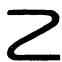
\includegraphics[keepaspectratio]{images/part002_3e739bde.jpg}}

我们可以证明，可度量化 Montel 空间 \(E\) 的强对偶当 \(E\) 是无限维时不是可度量化的（IV，第 57 页，习题 1）。

\section{FRÉCHET 空间的对偶}

\subsection{半桶型空间}

命题 1. --- 设 E 是一个局部凸空间。下列条件等价：

\begin{enumerate}
\def\labelenumi{(\roman{enumi})}
\item
  设 U 是 E 的一个子集，它吸收 E 的每个有界子集，且是 E 中凸、均衡且闭的零邻域的一个序列的交。则 U 是 E 中 0 的一个邻域。
\item
  对每个局部凸空间 \(\mathbf{F}\)，\(\mathcal{L}_{\mathfrak{b}}(\mathbf{E};\mathbf{F})\) 的每个作为可数个等度连续子集之并的有界子集都是等度连续的。
\item
  在 E 的强对偶 \(E_{b}^{\prime}\) 中，每个作为可数个等度连续子集之并的有界子集都是等度连续的。
\end{enumerate}

显然 (iii) 是 (ii) 的特殊情形。

\begin{enumerate}
\def\labelenumi{(\roman{enumi})}
\item
  \(\Rightarrow\) (ii)：设 H 是 \(\mathcal{L}_b(E;F)\) 的一个有界子集，\((\mathrm{H}_n)\) 是 \(\mathcal{L}_b(E;F)\) 的等度连续子集的一个序列，使得 \(\mathrm{H} = \bigcup_{n}\mathrm{H}_{n}\)。设 V 是 F 中凸、均衡且闭的零邻域。对每个 \(n\)，集 \(\mathrm{W}_n = \bigcap_{u\in \mathrm{H}_n}u^{-1}(\mathrm{V})\) 是 E 中凸、均衡且闭的零邻域，因为 \(\mathrm{H}_n\) 等度连续。集 \(\mathrm{W} = \bigcap_{u\in \mathrm{H}}u^{-1}(\mathrm{V})\) 吸收 E 的每个有界子集，因为 H 在 \(\mathcal{L}_b(E;F)\) 中有界（III，第 22 页），且我们有 \(\mathrm{W} = \bigcap_{n}\mathrm{W}_{n}\)。若 E 满足 (i)，则集 W 是 E 中 0 的一个邻域，故 H 等度连续。
\item
  \(\Rightarrow\) (i)：设 \((\mathrm{U}_n)\) 是 E 中凸、均衡且闭的零邻域的一个序列。我们假定集 \(\mathbf{U} = \bigcap_{n}\mathbf{U}_{n}\) 吸收 E 的每个有界子集，从而它的极集 \(\mathbf{U}^{\circ}\) 在 \(\mathbf{E}_b^\prime\) 中有界。于是集 \(\mathbf{B} = \bigcup_{n}\mathbf{U}_{n}^{\circ}\) 包含在 \(\mathbf{U}^{\circ}\) 中，从而在 \(\mathbf{E}_b^\prime\) 中有界。若 E 满足 (iii)，则集 B 在 \(\mathbf{E}'\) 中等度连续；于是 B 在 E 中的极集 \(\mathbf{B}^{\circ} = \bigcap_{n}(\mathbf{U}_{n}^{\circ})^{\circ} = \bigcap_{n}\mathbf{U}_{n} = \mathbf{U}\) 是 E 中 0 的一个邻域。
\end{enumerate}

定义 1. --- 若局部凸空间 E 满足命题 1 的等价条件，则称它是半桶型的。

每个桶型空间都是半桶型的。这对每个有界型空间也成立（III，第 22 页，命题 10）。

\subsection{局部凸可度量化空间的对偶}

命题 2. --- 设 E 是一个局部凸可度量化空间，F 是它的强对偶。空间 F 是完备的、半桶型的，且满足下列条件：

(DB) 存在有界子集的一个序列 \((\mathbf{A}_n)_{n\in \mathbb{N}}\)（\(\mathbf{F}\) 中的），使得 \(\mathbf{F}\) 的每个有界子集都包含在某个 \(\mathbf{A}_n\) 中。

空间 E 是有界型的（III，第 12 页，命题 2），从而它的强对偶是完备的（III，第 23 页，推论 1）。

设 \((\mathrm{V}_{n})_{n\in\mathbf{N}}\) 是 E 中零邻域的一个递减序列，使得 E 的每个零邻域都包含某个 \(V_{n}\)。设 \(A_{n}\) 是 \(V_{n}\) 在 F 中的极集。由于 E 是有界型的，F 的每个有界子集都等度连续（III，第 22 页，命题 10），从而包含在某个 \(A_{n}\) 中。换言之，空间 F 满足条件 (DB)。

我们现在证明 F 是半桶型的。设 \((\mathrm{U}_{n})_{n\in\mathbf{N}}\) 是 F 中凸、均衡且闭的零邻域的一个序列。我们假定集 \(U=\bigcap_{n}U_{n}\) 吸收 F 的每个有界子集。我们将证明 U 是 F 中 0 的一个邻域。为此，我们将对整数 \(n\geqslant0\) 用归纳法构造实数 \(\lambda_{n}>0\) 与 F 中凸、均衡的零邻域 \(W_{n}\)（它们对于 \(\sigma(\mathrm{F},\mathrm{E})\) 是闭的），使之满足下列关系

\[
\lambda_ {n} \mathrm{A} _ {n} \subset \frac {1}{2} \mathrm{U} \cap \left(\bigcap_ {0 \leqslant i <   n} \mathrm{W} _ {i}\right)\tag{1}
\]

\[
\bigcup_ {0 \leqslant i \leqslant n} \lambda_ {i} \mathrm{A} _ {i} \subset \mathrm{W} _ {n} \subset \mathrm{U} _ {n}.\tag{2}
\]

假定诸数 \(\lambda_{i}\) 与诸集 \(\mathrm{W}_i\) 已对 \(0 \leqslant i < n\) 构造出来。根据假设，集 U 吸收 F 的有界子集；此外，对 \(0 \leqslant i < n\)，\(\mathrm{W}_i\) 是 F 中 0 的一个邻域，从而吸收 F 的有界子集。因此可以找到满足 (1) 的数 \(\lambda_{n} > 0\)。设 C 表示对于 \(\sigma(\mathrm{F}, \mathrm{E})\) 而言 \(\bigcup_{0 \leqslant i \leqslant n} \lambda_i \mathrm{A}_i\) 的闭凸均衡包；集 C 是等度连续的，

从而对于 \(\sigma(\mathrm{F},\mathrm{E})\) 紧（III，第 17 页，推论 2）。由于 \(\mathrm{U}_n\) 是 F 中 0 的一个邻域，存在 E 的有界子集 B 使得 \(\mathbf{B}^{\circ}\subset\frac{1}{2}\mathbf{U}_{n}\)。令 \(\mathrm{W}_n=\mathrm{C}+\mathrm{B}^{\circ}\)。由于 \(\mathbf{B}^{\circ}\) 是 F 中 0 的一个邻域，我们看出 \(\mathrm{W}_n\) 是 F 中凸、均衡的零邻域。此外，C 紧且 \(\mathbf{B}^{\circ}\) 对于 \(\sigma(\mathrm{F},\mathrm{E})\) 闭；由 GT, III, § 4, 第 1 目的推论 1，\(\mathrm{W}_n\) 对于 \(\sigma(\mathrm{F},\mathrm{E})\) 闭。最后，我们有 \(\mathbf{C}\subset\frac{1}{2}\mathbf{U}\subset\frac{1}{2}\mathbf{U}_n\) 与 \(\mathbf{B}^{\circ}\subset\frac{1}{2}\mathbf{U}_n\)，从而 \(\mathrm{W}_n\subset\mathrm{U}_n\)，因为 \(\mathrm{U}_n\) 是凸的。这样我们就建立了 (2)。

令
\[
\mathrm{W} = \bigcap_ {n} \mathrm{W} _ {n}
\]

则
\[
\mathbf {W} \subset \mathbf {U}
\]

由 (1) 与 (2)，我们有
\[
\lambda_ {i} \mathrm{A} _ {i} \subset \mathrm{W} _ {j} \quad \text {for all } i \text { and } j
\]

在 N 中，从而 \(\lambda_{i}A_{i}\subset W\)（对所有 \(i\in N\)）。特别地，W 是吸收的，从而是对于 \(\sigma(\mathrm{F},\mathrm{E})\) 的一个桶。由 IV 第 4 页的注 3，W 是 F 中 0 的一个邻域。更加地，U 是 F 中 0 的一个邻域，故 F 是半桶型的。

下列推论把 Banach-Steinhaus 定理推广到 Fréchet 空间的对偶（参见 III，第 25 页，推论 2）。

推论. --- 设 G 是一个 Hausdorff 局部凸空间，\((u_{n})\) 是从 F 到 G 中的线性映射的一个序列，它简单收敛于一个从 F 到 G 中的映射 u。则 u 连续，且序列 \((u_{n})\) 在 F 的每个预紧子集上一致收敛于 u。

由于 F 是完备的，所有 \(u_{n}\) 组成的集（它对于简单收敛拓扑有界）在 \(\mathcal{L}_{b}(F;G)\) 中有界（III，第 27 页，推论 1）。由于空间 F 是半桶型的（命题 2），\(\mathcal{L}_{b}(F;G)\) 的每个可数且有界的子集由 IV 第 21 页的命题 1 都是等度连续的。因此诸 \(u_{n}\) 组成的集等度连续，且推论由 III 第 18 页的推论得出。

\subsection{局部凸可度量化空间的双对偶}

命题 3. --- 设 E 是一个局部凸可度量化空间，\(E_{b}^{\prime}\) 是它的强对偶，G 是一个 Fréchet 空间。空间 \(\mathcal{L}_{b}(E_{b}^{\prime}; G)\) 是 Fréchet 空间。

由（IV，第 22 页的）命题 2，存在有界子集的一个序列 \((\mathrm{A}_n)\)（\(\mathrm{E}_b'\) 中的），使得 \(\mathrm{E}_b'\) 的每个有界子集都包含在某个 \(\mathrm{A}_n\) 中。设 \((\mathrm{V}_n)\) 是 \(\mathbf{G}\) 中零邻域的一个可数基本系。设 \(\mathrm{H}_{mn}\) 是线性映射 \(u\)（从 \(\mathrm{E}_b'\) 到 \(\mathbf{G}\) 中的，且满足 \(u(\mathrm{A}_m) \subset \mathrm{V}_n\)）组成的集。则 \((\mathrm{H}_{mn})\) 是 \(\mathcal{L}_b(\mathrm{E}_b'; \mathrm{G})\) 中零邻域的一个基本系，从而后一空间是可度量化的。

为证明 \(\mathcal{L}_b(\mathrm{E}_b';\mathbf{G})\) 完备，只需证明此空间中每个 Cauchy 序列 \((u_n)\) 都收敛；由于 \(\mathbf{G}\) 完备，存在线性映射 \(u:\mathrm{E}_b' \to \mathbf{G}\) 使得 \((u_n)\) 简单收敛于 \(u\)。由 IV 第 23 页的推论，我们有 \(u \in \mathcal{L}_h(\mathrm{E}_h';\mathbf{G})\)。于是由 GT, X, § 1, 第 5 目的命题 5，\((u_n)\) 收敛于 \(u\)（在 \(\mathcal{L}_b(\mathrm{E}_b';\mathbf{G})\) 中）。

推论. --- 局部凸可度量化空间的双对偶是 Fréchet 空间。

\subsection{自反 Fréchet 空间的对偶}

命题 4. --- 设 E 是一个自反 Fréchet 空间。E 的强对偶 \(E_{b}^{\prime}\) 是 Banach 空间的一个序列的归纳极限。

设 \((\mathrm{V}_{n})_{n\in\mathbf{N}}\) 是 E 中凸、均衡且闭的零邻域的一个递减序列，使得 E 的每个零邻域都包含某个 \(V_{n}\)。设 \(A_{n}\) 是 \(V_{n}\) 在 \(E'\) 中的极集。则 \(A_{n}\) 是凸、均衡且对于 \(\sigma(\mathrm{E}',\mathrm{E})\) 紧的；由 III 第 8 页的推论，空间 \(E_{A_{n}}'\) 是 Banach 空间。我们将证明 \(E_{b}'\) 是诸空间 \(E_{A_{n}}'\) 的归纳极限；换言之，\(E'\) 的每个吸收诸 \(A_{n}\) 中每一个的凸、均衡子集 U 都是 \(E_{b}'\) 中 0 的一个邻域。对每个 \(n\in\mathbf{N}\)，选取实数 \(\lambda_{n}>0\) 使得 \(\lambda_{n}A_{n}\subset U\)。设 \(B_{n}\) 是集 \(\bigcup_{0\leqslant i\leqslant n}\lambda_{i}A_{i}\) 的凸包；令 \(V=\bigcup_{n}B_{n}\)，则 \(V\subset U\)。对每个 \(n\in\mathbf{N}\)，集 \(B_{n}\) 是凸、均衡且对于 \(\sigma(\mathrm{E}',\mathrm{E})\) 紧的（II，第 14 页，命题 15）。

现在我们将证明 \(\frac{1}{2}\mathrm{V}^{\circ \circ}\subset \mathrm{V}\)。设 \(x\in \mathrm{E}_b^\prime -\mathrm{V}\)；对每个 \(n\in \mathbf{N}\)，我们有 \(x\notin \mathbf{B}_n\)，且由于 \(\mathbf{B}_n\) 对于 \(\sigma (\mathrm{E}',\mathrm{E})\) 闭，存在元素 \(y_{n}\)（在 \(\mathbf{B}_n^\circ\) 中的）使得 \(\langle y_n, x \rangle = 1\)（II，第 38 页，命题 4）。由于 E 是自反的，E 的每个有界子集对于 \(\sigma(E, E')\) 相对紧（IV，第 16 页，定理 2）。由 \(B_n\) 的定义，我们有

\[
\lambda_ {i} y _ {n} \in \mathrm{V} _ {i} \quad \text { for   all } \quad n \geqslant i  ,\tag{3}
\]

从而序列 \((y_{n})\) 有界。设 \(y\) 是 \((y_{n})\) 对于拓扑 \(\sigma(\mathrm{E},\mathrm{E}')\) 的一个极限点。我们有 \(y\in\mathrm{V}^{\circ}=\bigcap_{n}\mathrm{B}_{n}^{\circ}\) 且 \(\langle y,x\rangle=1\)。于是 \(x\notin\frac{1}{2}\mathrm{V}^{\circ\circ}\)，从而有包含关系 \(\frac{1}{2}\mathrm{V}^{\circ\circ}\subset\mathrm{V}\)，更加有 \(\frac{1}{2}\mathrm{V}^{\circ\circ}\subset\mathrm{U}\)。

由于 \(E_{b}^{\prime}\) 的每个有界子集都包含在某个集 \(A_{n}\) 中，集 \(V = \bigcup_{n} B_{n}\)

吸收 \(E_{b}^{\prime}\) 的每个有界子集。于是，\(V^{\circ}\) 在 E 中有界，从而 \(\frac{1}{2}V^{\circ\circ}\) 是 \(E_{b}^{\prime}\) 中 0 的一个邻域。更加地，U 是 \(E_{b}^{\prime}\) 中 0 的一个邻域。

推论. --- 自反 Fréchet 空间的强对偶是有界型的且是桶型的。

Banach 空间的归纳极限按定义是有界型的。此外，Banach 空间是桶型的（III，第 25 页，推论），且桶型空间的每个归纳极限都是桶型空间（III，第 25 页，推论 3）。

\subsection{Fréchet 空间对偶上的紧收敛拓扑}

定理 1（Banach-Dieudonné）. --- 设 E 是一个局部凸可度量化空间。下列拓扑在 E 的对偶 E' 上一致：

\begin{enumerate}
\def\labelenumi{\alph{enumi})}
\item
  拓扑 \(\mathcal{T}_{\mathfrak{N}}\)（\(\mathfrak{N}\)-收敛的），其中 \(\mathfrak{N}\) 是 \(E\) 的这样的子集组成的族：每个子集由一个收敛于 0 的序列的点组成；
\item
  在 E 的紧子集上一致收敛的拓扑 \(\mathcal{T}_{\mathrm{c}}\)；
\item
  在 E 的预紧子集上一致收敛的拓扑 \(\mathcal{T}_{pc}\)；
\item
  拓扑 \(\mathcal{T}_f\)，它是这样的最细拓扑：在每个等度连续子集上诱导出与 \(\sigma(\mathrm{E}',\mathrm{E})\) 相同的拓扑（这些子集属于 \(\mathrm{E}'\)）。
\end{enumerate}

首先注意到，\(E'\) 的子集 A 对于 \(T_{f}\) 闭，当且仅当 \(A \cap H\) 对于 \(\sigma(E', E)\) 闭（对每个子集 H，它属于 \(E'\)、等度连续且对于 \(\sigma(E', E)\) 闭）。弱拓扑 \(\sigma(E', E)\) 与 \(T_{pc}\) 在 \(E'\) 的每个等度连续子集上诱导出相同的拓扑（III，第 17 页，命题 5）。因此，拓扑 \(T_{R}\)、\(T_{c}\)、\(T_{pc}\)、\(T_{f}\) 中的每一个都比它后面一个粗。于是只需证明 \(T_{R}\) 比 \(T_{f}\) 细。此外，\(E'\) 中的每个平移对于 \(T_{f}\) 是一个同胚。因此只需证明：若 F 是 \(E'\) 的一个对于 \(T_{f}\) 闭且不包含 0 的子集，则存在集 \(S \in R\) 使得 \(S^{\circ} \cap F = \varnothing\)。

设 \((\mathbf{U}_{n})_{n\geqslant0}\) 是 E 中零邻域的一个递减序列，构成零邻域的一个基本系。我们将对 \(n\geqslant0\) 用归纳法构造有限集 \(X_{n}\)，使得我们有

\[
\mathrm{X} _ {n} \subset \mathrm{U} _ {n}\tag{4}
\]

\[
\left(\bigcup_ {0 \leqslant p \leqslant n} \mathrm{X} _ {p}\right) ^ {\circ} \cap \mathrm{U} _ {n + 1} ^ {\circ} \cap \mathrm{F} = \varnothing\tag{5}
\]

对每个整数 \(n \geqslant 0\)。设 \(m \geqslant 0\) 是这样的整数：\(X_{n}\) 已对 \(0 \leqslant n < m\) 构造出来，且对 \(0 \leqslant n < m\) 满足 (4) 与 (5)。对每个 \(x \in U_{m}\)，令

\[
\mathrm{F} _ {x} = \big (\bigcup_ {0 \leqslant p <   m} \mathrm{X} _ {p} \big) ^ {\circ} \cap \{x \} ^ {\circ} \cap \mathrm{U} _ {m + 1} ^ {\circ} \cap \mathrm{F}.
\]

取 \(n = m - 1\) 的公式 (5) 蕴含 \(\bigcap_{x\in \mathrm{U}_m}\mathrm{F}_x = \emptyset\)。此外，集 \(\mathrm{U}_{m + 1}^{\circ}\) 是等度连续的，且对于 \(\sigma (\mathrm{E}',\mathrm{E})\) 紧。鉴于 \(\mathcal{T}_f\) 的定义，每个集 \(\mathrm{F}_x\) 对于 \(\sigma (\mathrm{E}',\mathrm{E})\) 紧；因此存在有限子集 \(\mathrm{X}_m\)（\(\mathrm{U}_m\) 中的）使得 \(\bigcap_{x\in \mathrm{U}_m}\mathrm{F}_x = \emptyset\)，即关系 (5) 对 \(n = m\) 满足。

令 \(S = \bigcup_{n\geqslant 0}X_n\)。我们有 \(X_{n}\subset U_{p}\)（对 \(n\geqslant p\)），因此 \(S\) 是 \(E\) 中一个收敛于 0 的序列的点组成的集。由 (5) 我们推出 \(S^{\circ}\cap U_{n + 1}^{\circ}\cap F = \emptyset\)，且由于 \(E'\) 是诸集 \(U_{n + 1}^{\circ}\) 组成的序列之并，我们得到 \(S^{\circ}\cap F = \emptyset\)。

推论 1. --- 设 E 是一个局部凸可度量化空间。E 的每个预紧子集都包含在一个收敛于 0 的序列的点组成的集的闭凸均衡包中。

这由拓扑 \(\mathcal{T}_{pc}\) 与 \(\mathcal{T}_{\mathfrak{N}}\) 相同这一事实得出，依据是 III 第 15 页的命题 2。

推论 2. --- 设 E 是一个 Fréchet 空间。为使 E 的对偶 E' 的凸子集 A 对于 \(\sigma(E', E)\) 闭，必要且充分的是 \(A \cap U^{\circ}\) 对于 \(\sigma(E', E)\) 闭（对 E 中 0 的每个邻域 U）。

由于 E 完备，拓扑 \(T_{c}\) 在 \(E'\) 上与 \(E'\) 和 E 之间的对偶相容（IV，第 3 页，例）；因此 \(E'\) 中的闭凸子集对于 \(T_{c}\) 与 \(\sigma(E', E)\) 是相同的（IV，第 1 页，命题 1）。于是推论由拓扑 \(T_{c}\) 与 \(T_{f}\) 的相同性得出。

回忆（I，第 13 页）：E' 中对于 \(\sigma(\mathrm{E}', \mathrm{E})\) 闭的超平面是 E' 上由 E 的元素所对应的线性型的核。因此推论 2 给出了 III 第 21 页的推论 1（对 Fréchet 空间而言）的另一个证明。

推论 3. --- 设 E 是一个 Banach 空间，M 是 E 的对偶 E' 的一个向量子空间。为使 M 对于弱拓扑 \(\sigma(E', E)\) 闭，必要且充分的是它与 E' 中（闭）单位球的交对于 \(\sigma(E', E)\) 闭。

例. --- * 设 H 是一个满足第一可数公理的 hilbertian 空间；设 \(H_{\sigma}\) 表示赋以弱化拓扑的空间 H。设 \(\mathcal{L}^{1}(H)\) 是 H 的核型自同态组成的 Banach 空间（V，第 51 页，及 TS，V）；\(\mathcal{L}^{1}(H)\) 中的范数由 \(\|u\|_{1} = \operatorname{Tr}((u^{*}u)^{1/2})\) 定义。我们可以把 \(\mathcal{L}(H)\) 等同于 Banach 空间 \(\mathcal{L}^{1}(H)\) 的对偶，方法是把线性型 \(\phi_{u}: v \mapsto \operatorname{Tr}(uv)\)（\(\mathcal{L}^{1}(H)\) 上的）与每个 \(u \in \mathcal{L}(H)\) 相对应。设 A 是 \(\mathcal{L}(H)\) 的一个子代数，包含 1 且在 \(u \mapsto u^{*}\) 下稳定；它是 von Neumann 代数当且仅当它在 \(\mathcal{L}(H)\) 中对于弱拓扑 \(\sigma(\mathcal{L}(H), \mathcal{L}^{1}(H))\) 闭。由推论 3，我们推出下列判别法：为使 A 是 von Neumann 代数，必要且充分的是：若 \((u_{n})\) 是 A 中范数 \(\leqslant 1\) 的元素的任一序列，在空间 \(\mathcal{L}_{s}(H; H_{\sigma})\) 中有极限 u，则 u 属于 A。

\subsection{分别连续的双线性映射}

引理 1. --- 设 E 与 F 是两个局部凸可度量化空间，u 是从 \(E_{b}^{\prime}\) 到 F 中的一个连续线性映射。则存在 \(E_{b}^{\prime}\) 中 0 的一个邻域，它在 u 下的像在 F 中有界。

设 \((\mathrm{U}_n)_{n\in \mathbf{N}}\)（相应地，\((\mathrm{V}_n)_{n\in \mathbf{N}}\)）是 E（相应地，F）中零邻域的一个基本系。我们假定诸集 \(\mathrm{U}_n\) 是均衡的且构成一个递减序列。由于 \(u\) 连续，对每个 \(n\in \mathbf{N}\)，存在 E 中的有界集 \(\mathrm{B}_n\) 使得 \(u(\mathrm{B}_n^\circ)\subset \mathrm{V}_n\)。由于 \(\mathrm{B}_n\) 有界，存在实数 \(\lambda_n > 0\) 使得 \(\lambda_{n}\mathrm{B}_{n}\subset \mathrm{U}_{n}\)。令 \(\mathrm{B} = \bigcup_{n\in \mathbf{N}}\lambda_n\mathrm{B}_n\)。

我们将证明集 B 在 E 中有界，换言之，对每个整数 \(m \geqslant 0\)，存在实数 \(\mu > 0\) 使得 \(\mu B \subset U_{m}\)。由于诸集 \(B_{n}\) 有界，存在实数 \(\mu\) 使得 \(0 < \mu \leqslant 1\) 且 \(\mu \cdot (\lambda_{n} B_{n}) \subset U_{m}\)（对 \(0 \leqslant n \leqslant m\)）；我们还有 \(\lambda_{n} B_{n} \subset U_{n} \subset U_{m}\)（若 n \textgreater{} m）；从而 \(\mu B \subset U_{m}\)，因为 \(U_{m}\) 是均衡的。

设 \(\mathbf{U}\) 是 \(\mathbf{B}\) 在 \(\mathrm{E}_b'\) 中的极集。它是 \(\mathrm{E}_b'\) 中 0 的一个邻域，且我们有 \(\lambda_n\mathrm{B}^\circ \subset \mathrm{B}_n^\circ\)，从而 \(\lambda_n u(\mathrm{U}) \subset \mathrm{V}_n\)（对所有 \(n \in \mathbf{N}\)）。于是 \(u(\mathrm{U})\) 在 \(\mathrm{F}\) 中有界。

定理 2. --- 设 \(E_{1}\) 与 \(E_{2}\) 是两个自反 Fréchet 空间，G 是一个局部凸 Hausdorff 空间。对 i = 1, 2，设 \(F_{i}\) 是 \(E_{i}\) 的强对偶。则每个分别连续的双线性映射 \(u: F_{1} \times F_{2} \to G\) 都连续。

空间 G 同构于 Banach 空间的一个乘积的子空间（II，第 5 页，命题 3）。因此在附加假设 G 是 Banach 空间之下证明定理就够了。但 \(F_{1}\) 是桶型的且 \(F_{2}\) 是有界型的（IV，第 24 页，推论），且 \(\mathcal{L}_{b}(F_{2}; G)\) 是 Fréchet 空间（IV，第 23 页，命题 3）。设 v 表示由 u 按下列关系式所对应的、从 \(F_{1}\) 到 \(\mathcal{L}_{b}(F_{2}, G)\) 中的线性映射：

\[
u (x _ {1}, x _ {2}) = v (x _ {1}) \left(x _ {2}\right) \quad \left(x _ {1} \in \mathrm{F} _ {1}, x _ {2} \in \mathrm{F} _ {2}\right).
\]

由于 \(F_{1}\) 是桶型的且 u 分别连续，v 连续（III，第 31 页，命题 6）。由于 v 连续，引理 1 蕴含存在 0 的一个邻域 \(U_{1}\)（\(F_{1}\) 中的），它在 v 下的像在 \(\mathcal{L}_{b}(F_{2}; G)\) 中有界。换言之，对每个有界子集 \(B_{2}\)（\(F_{2}\) 中的），集 \(u(U_{1} \times B_{2})\) 在 Banach 空间 G 中有界。设 \(U_{2}\) 是所有这样的 \(x_{2} \in F_{2}\) 组成的集：它们满足 \(\|u(x_{1}, x_{2})\| \leqslant 1\)（对所有 \(x_{1} \in U_{1}\)）。则集 \(U_{2}\) 吸收每个有界子集；由于 \(F_{2}\) 是有界型的，\(U_{2}\) 是 \(F_{2}\) 中 0 的一个邻域，这就证明了 u 连续。

\section{FRÉCHET 空间的严格态射}

对每个局部凸空间 E，设 S(E) 表示 E 上所有连续半范数组成的集。对每个 \(p \in \mathrm{S}(\mathrm{E})\)，设 \(H_{p}\) 表示 E 上所有满足 \(|f| \leqslant p\) 的线性型 f 组成的集。族 \((\mathrm{H}_{p})_{p \in \mathrm{S}(\mathrm{E})}\) 是由 \(E'\) 的等度连续子集组成的有界结构的一个基。

\subsection{严格态射的刻画}

命题 1. --- 设 E 与 F 是两个局部凸空间，u 是从 E 到 F 中的一个连续线性映射。为使 u 是严格态射，必要且充分的是满足下列条件：

(MS) 对每个半范数 \(p \in \mathrm{S}(\mathrm{E})\)（在 \(u\) 的核上为零的），存在 \(q\)（\(\mathrm{S}(\mathrm{F})\) 中的）使得 \(p \leqslant q \circ u\)。

设 N 是 u 的核，M 是 u 的像；我们引入 u 的典范分解，即

\[
\mathrm{E} \xrightarrow {\pi} \mathrm{E} / \mathrm{N} \xrightarrow {\tilde {u}} \mathrm{M} \xrightarrow {\iota} \mathrm{F}.
\]

E 上在 N 上为零的连续半范数是半范数 \(p_{1} \circ \pi\)（其中 \(p_{1}\) 取遍 S(E/N)）；类似地，S(M) 由这样的半范数 \(q_{1}\) 组成：存在 \(q \in \mathrm{S}(F)\) 使得 \(q_{1} \leqslant q/F\)。最后，u 是严格态射当且仅当双射连续线性映射 \(\tilde{u}\) 有连续的逆；这也就是说 S(E/N) 中的每个半范数都具有形式 \(q_{1} \circ \tilde{u}\)（其中 \(q_{1}\) 属于 S(M)）。命题 1 立即由这些注记得出。

命题 2. --- 设 E 与 F 是两个 Hausdorff 局部凸空间，u 是从 E 到 F 中的一个连续线性映射。为使 u 是严格态射，必要且充分的是它的转置 \({}^t u\): F' → E' 满足下列条件：

\begin{enumerate}
\def\labelenumi{\alph{enumi})}
\item
  \(^{t}u\) 的像在 \(E'\) 中对于 \(\sigma(E', E)\) 闭。
\item
  \(\mathbf{E}'\) 的每个等度连续子集，若包含在 \({}^t u\) 的像中，就是 \({}^t u\) 对 \(\mathbf{F}'\) 的某个等度连续子集所取的像。
\end{enumerate}

若如此，我们有 \(\operatorname{Ker}^t u = (\operatorname{Im} u)^\circ\) 与 \(\operatorname{Im}^t u = (\operatorname{Ker} u)^\circ\)，且存在从 \(\operatorname{Coker}^t u\) 到 \(\operatorname{Ker} u\) 的对偶上的以及从 \(\operatorname{Ker}^t u\) 到 \(\operatorname{Coker} u\) 的对偶上的典范同构。

设 N 是 u 的核，I 是 u 的像。由 II 第 47 页的推论 2，\(^{t}u\) 的核是 I 的正交，而 \(^{t}u\) 的像对于 \(\sigma(E', E)\) 的闭包是 N 的正交 \(N^{\circ}\)。于是 a) 与 b) 的合取等价于下列条件：

b') \(E'\) 的每个包含在 \(N^{\circ}\) 中的等度连续子集都是 \(^{t}u\) 对 \(F'\) 的某个等度连续子集所取的像。

由于 \(N^{\circ}\) 可以等同于 E/N 的对偶，IV 第 8 页的命题 9 (i) 表明：\(E'\) 的包含在 \(N^{\circ}\) 中的等度连续子集就是包含在形如 \(H_{p}\) 的集中的那些集，其中 p 是 E 上的连续半范数且在 N 上为零。于是条件 \(b')\) 说的是：对每个在 N 上为零的半范数 \(p \in \mathrm{S}(\mathrm{E})\)，存在 \(q \in \mathrm{S}(\mathrm{F})\) 使得 \(\mathrm{H}_{p} \subset {}^{t}u(\mathrm{H}_{q})\)。由 Hahn-Banach 定理（II，第 23 页，推论 1 与第 63 页，定理 1 与推论 1），我们有 \(u(\mathrm{H}_{q}) = \mathrm{H}_{q \circ u}\)，且关系 \(H_{p} \subset H_{p'}\) 与 \(p \leqslant p'\) 对所有半范数 p 与 \(p'\)（S(E) 中的）等价。因此关系 \(H_{p} \subset {}^{t}u(\mathrm{H}_{q})\) 等价于关系 \(p \leqslant q \circ u\)。由命题 1，性质 \(b')\) 蕴含 u 是严格态射。

假定 \(u\) 是严格态射。我们已看到，\(^t u\) 的核是 I 的正交，而 \(^t u\) 的像是 N 的正交。u 的余核是空间 F/I，它的对偶可以等同于 \(I^{\circ} = Ker^{t}u\)。类似地，N = Ker u 的对偶可以等同于 \(E^{\prime}/N^{\circ}\)（IV，第 8 页），即等同于 \(^{t}u\) 的余核，因为 \(N^{\circ}\) 是 \(^{t}u\) 的像。

注. --- 采用命题 2 的记号，性质 \(b'\) ) 还蕴含 \(u\) 对于弱化拓扑是严格态射（II，第 49 页，推论 3）。

命题 3. --- 设 E 与 F 是两个局部凸空间，u 是从 E 到 F 中的一个连续线性映射。我们假定 E 是 Hausdorff 的且 F 是可度量化的。为使 u 是严格态射，必要且充分的是 \({}^t u\) 的像在 E' 中对于弱拓扑 \(\sigma(E', E)\) 闭。

必要性由命题 2 得出。

反之，假定 \(^t u\) 的像对于 \(\sigma(E', E)\) 闭，并如命题 1 的证明中那样引入 \(u\) 的典范分解。由上述注记，逆映射 \(\tilde{u}^{-1}\)（\(\tilde{u}\) 的）对于弱化拓扑连续。但 F 的子空间 \(M = u(E)\) 是可度量化的，从而是有界型的（III，第 12 页，命题 2）；于是（IV，第 7 页，命题 7 (ii)），\(\tilde{u}^{-1}\) 连续，故 \(u\) 是严格态射。
